\documentclass[aoas,preprint]{imsart}
%\documentclass[11pt]{extarticle}
%\RequirePackage{mdframed}
%\usepackage{mdframed}
\usepackage[framemethod=TikZ]{mdframed}
\RequirePackage[OT1]{fontenc}
\usepackage[utf8x]{inputenc}
\RequirePackage{amsthm,amsmath}
\RequirePackage{natbib}
\RequirePackage[colorlinks,citecolor=blue,urlcolor=blue]{hyperref}
\usepackage[margin=0.5in]{geometry}

\usepackage[sc]{mathpazo}
\usepackage{amsmath, wrapfig}
\usepackage{dsfont}
\usepackage{graphicx}
\usepackage{caption}
\DeclareCaptionFormat{myformat}{\hrulefill \\ #1#2#3}
\DeclareCaptionFont{small}{\footnotesize}
\DeclareCaptionFont{blue}{\color{blue}} 
\DeclareCaptionFont{bf}{\bfseries}

\renewcommand{\figurename}{Supplementary Figure}
\renewcommand{\thefigure}{S\arabic{figure}}
\renewcommand{\tablename}{Supplementary Table}
\renewcommand{\thetable}{S\arabic{table}}
\captionsetup[figure]{format=myformat,labelfont={blue,bf,small},font=small}
\usepackage{booktabs}% http://ctan.org/pkg/booktabs

%\usepackage{algorithm,algcompatible,amsmath}
\usepackage{algorithm, eqparbox,array}% http://ctan.org/pkg/algorithms
\usepackage{algpseudocode}% http://ctan.org/pkg/algorithmicx
%\usepackage{xcolor}
%\usepackage[usenames, dvipsnames]{color}
\usepackage{color}
\RequirePackage{xcolor}
%\usepackage{mdframed}




\setlength{\parskip}{1ex}
\newtheorem{lemma}{Lemma}
\newtheorem{theorem}{Theorem}
\newtheorem{prop}{Proposition}
\DeclareGraphicsRule{.tif}{png}{.png}{`convert #1 `dirname #1`/`basename #1 .tif`.png}

\begin{document}

\large
\centerline{\bf Supplementary Material }

\noindent
Main document: {\em A compositional model to assess expression changes from single-cell RNA-seq data}

\vspace{.2in}
\noindent
Authors: Ma, Korthauer, Kendziorski, and Newton

\vspace{.2in}
\noindent
Version: May 5, 2019

\vspace{.4in}

\noindent
This supplement is organized to match the sectioning of the main document.   In summary,

\begin{enumerate}
\item Introduction
   \begin{itemize}
   %\item DEC vs EC data analysis
   \item R package
   \end{itemize}
\item Modeling
 \begin{itemize}
  \item Data Structure, Sampling Model, and Parameters
    \begin{list}{}{}
    \item Proof of Theorem 2
    \end{list}
  \item Method Structure and Clustering 
    \begin{list}{}{}
    \item \verb+EBSeq+
    \item \verb+modalClust+
    \item Randomized $K-$means
    \item Selecting $K$
    \end{list}
  \item Double Dirichlet Mixture
    \begin{list}{}{}
    \item Proof of Properties 1-6 and Theorem 3
    \end{list}
  \end{itemize}
\item Numerical Experiments
   \begin{itemize}
   \item Synthetic data, \verb+splatter+
   \item Empirical study, \verb+conquer+ and Null case
   \item Robustness
   \end{itemize}
\item Posterior consistency
  \begin{itemize}
   \item proof of theorem 4
  \end{itemize}
\end{enumerate}


\clearpage

\section{Introduction}

%\subsection{DEC vs EC}

%Using data from GSE75748, comparing conditions DEC vs EC.
%We have genes potentially to be DD uniquely identified by scDDboost. (supplementary Fig 1)

%\begin{figure}[h!]
%  \includegraphics[ width = 0.8\textwidth]{Figs/density_DECEC_DD.pdf}
%  \caption{Potentially to be DD genes uniquely identified by us. }
%  \label{fig:4}
%\end{figure}


\subsection{R package}

Reference can be found at github site ...

**on scDDboost, web page, etc**

\section{Modeling}

\subsection{Data Structure, Sampling Model, and Parameters}


Proof of Theorem 2.

\begin{proof}
Recall $\theta = (\phi, \psi, \mu, \sigma)$.
Through the sampling procedure of our model (Figure 3), assuming we known number of cells within each conditions $(n_1,n_2)$. We have $z^1, z^2$ are multinomial draw given $\phi$ and $\psi$, 
thus the generation of $y, z$ only depends on $(\phi,\psi)$
Also given $z$, $X_{g,c}$ is sampled through $\text{NB}(\mu_{g,z_c}, \sigma_g)$, only depends on $(\mu, \sigma)$.
Thus $P(X,y,z | \theta) = P(y, z | \phi,\psi ) P(X | z, \mu, \sigma)$, and we independently give priors for $(\mu,\sigma)$ and $(\phi, \psi)$
By the Baye's rule, 
\begin{align*}
P(\theta | X,y,z) &\propto P(X,y,z | \theta) P(\theta) \\
P(X,y,z | \theta) P(\theta)  &=  P(y, z | \phi,\psi ) P(X | z, \mu, \sigma) P(\mu,\sigma | z) P(\phi, \psi)\\
P(\phi,\psi | y, z) &\propto P(y, z | \phi,\psi )P(\phi, \psi)\\
P(\mu, \sigma | X, z) &\propto P(X | z, \mu, \sigma) P(\mu,\sigma | z)\\
\text{Thus }
P(\theta | X,y,z) &\propto P(\phi,\psi | y, z) P(\mu, \sigma | X, z)
\end{align*}
From this we know\\
1. Given $X,y$ and $z$, $(\phi, \psi) \perp (\mu, \sigma)$\\ 
2. Given condition and subtypes label $y,z$, $(\phi,\psi)$ is independent with $X$\\
3. Given $X$ and $z$, $(\mu, \sigma)$ is independent with $y$\\
Thus we have $  P\left(A_\pi \cap M_{g,\pi} |X,y,z \right) 
 =  P\left(A_\pi |y,z \right) \, 
                      P\left(M_{g,\pi}| X,z \right).  $
\end{proof}


\subsection{Method Structure and Clustering}

\subsubsection{EBSeq}
In this subsection, we go through how we implement and modified \texttt{EBSeq} to get $P(M_{g,\pi} | X, z)$.

Suppose we have $K$ subtypes, let $X_g^I = X_{g, 1}^I, ... , X_{g, S_1}^I$ denote transcripts at gene $g$ from subtype $I, I = 1, ... K$.  In the \texttt{EBSeq}, it assumed that counts within subtype $I$ are distributed as Negative Binomial:
$X_{g, s}^I | r_{g,s}, q_g^I \sim NB(r_{g,s}, q_g^I)$. Due to sample specific sizefactor in the raw counts, r is made sample specific. However, we are dealing with normalized counts rather than raw counts in \texttt{EBSeq}, We make $r$ shared at gene level across all samples, i.e. 
$X_{g, s}^I | \sigma_g, q_g^I \sim NB(\sigma_g, q_g^I)$

\begin{eqnarray*}
P(X_{g,s}^I | \sigma_g, q_g^I ) = {X_{g,s} + \sigma_g - 1 \choose X_{g,s} }(1 - q_g^I)^{X_{g,s}^I} (q_g^I)^{\sigma_g}
\end{eqnarray*}
and $\mu_{g,s}^I = \sigma_g(1 - q_g^I) / q_g^I$; For the ease of later deriving the density kernel $f$, we use $q$ rather than $\mu$ to parameterize the NB.  %\sigma_{g,s}^I = r_{g,s}(1 - q_g^I)/ (q_g^I)^2.$

From \texttt{EBSeq}, we assumed a prior distribution on $q_g^I : q_g^I | \alpha, \beta^{g} \sim Beta(\alpha, \beta^{g}).$ The hyperparameter $\alpha$ is shared by whole genome and $\beta^{g}$ is gene specific.
 

We force the size factor to be 1 for all cells and use the same procedure from \texttt{EBSeq} to estimate number of failure parameter $\sigma_g$. Namely, we have\\
1. gene-level sample mean $m_g = \frac{1}{n}\sum_{s = 1}^n X_{g,s}$, where $n = n_1 + n_2$ is the total number of cells \\
2. average of sample variances over subtypes $v_g = \frac{1}{K} \sum_{I = 1}^K v_g^I$.\\
3. $v_g^I$ is the unadjusted sample variance for subtype $I$, i.e. $v_g^I = \frac{1}{n^I}\sum_{s, z_s = I} (X_{g,s} - m_g^I)^2$ with $m_g^I$ is the sample mean within subtype $I$ and $n^I$ is the number of cells within subtype $I$.\\
We estimate pooled over-dispersion rate by $o_g = \frac{v_g}{m_g}$ and obtain $\sigma_g = m_g \frac{o_g}{1 - o_g}$ from the first moment of NB\\
Our target is to quantify the expression pattern between $K$ groups, 

\begin{eqnarray*}
M_{g,\pi} = \{ \theta \in \Theta: \; \mu_{g,k} = \mu_{g,k'} \iff k,k' \in b, b \in \pi \}.
\end{eqnarray*}



For example $K = 3$, there are 5 expression pattern, $P_1, P_2, ..., P_5$, Comparison between $\mu$ is equivalent as comparison between $q$.

\begin{align*}
&P1: q_g^1 = q_g^2 = q_g^3\\
&P2: q_g^1 = q_g^2 \neq q_g^3\\
&P3: q_g^1 \neq q_g^2 = q_g^3\\
&P4: q_g^1 = q_g^3 \neq q_g^2\\
&P5: q_g^1 \neq q_g^2 \neq q_g^3 \text{ and } q_g^1 \neq q_g^3
\end{align*}

Under the assumption that two groups $I$ and $J$ share the same $q_g$ we can pool the counts from the two groups by viewing them sampled from same distribution i.e. $X_g^{I, J} | \sigma_{g}, q_g \sim NB(\sigma_{g}, q_g)$, $q_g | \alpha, \beta^{g} \sim \text{Beta}(\alpha, \beta^{g})$ and obtained the prior predictive function $f(X_g^{I,J}) = \int_0 ^1 P(X_g^{I,J} | r_{g}, q_g) * P(q_g | \alpha, \beta^{g}) dq_g = \Big[ \overset{S}{\underset{s = 1}{\prod}} {X_{g,s} + \sigma_{g} - 1 \choose X_{g,s}} \Big] \frac{Beta(\alpha + \Sigma_{s = 1}^S \sigma_{g}, \beta^{g} + \Sigma_{s = 1}^S X_{g,s})}{Beta(\alpha, \beta^{g})}$.  Consequently, we have prior predictive function for $P1, ..., P5$ as


\begin{align*}
&h_1^{g}(X_g) = f(X_g^{1,2,3})\\
&h_2^{g}(X_g) = f(X_g^{1,2})f(X_g^3)\\
&h_3^{g}(X_g) = f(X_g^1)f(X_g^{2,3})\\
&h_4^{g}(X_g) = f(X_g^{1,3})f(X_g^2)\\
&h_5^{g}(X_g) = f(X_g^1)f(X_g^2)f(X_g^3)\\
\end{align*}

where $h_i^{g}(X_g)$ = $P(X_g | M_{g,\pi_i},z)$ for associated $\pi_i$.
Then the marginal distribution of counts $X_g$ is $\overset{5}{\underset{k = 1}{\Sigma}} p_k h_k^{g}(X_g)$, 
where the marginal $p_k = P(M_{g,\pi} | z)$(shared by all genome). Thus, the posterior probability of an expression pattern $k$ is obtained by:
\begin{eqnarray*}
\frac{p_k h_k(X_g)}{\overset{5}{\underset{k = 1}{\Sigma}} p_k h_k^{g}(X_g)}
\end{eqnarray*}


In the optimization steps for determining the hyper parameters $(\alpha, \beta^g, p)$, the computation and memory increase exponentially with the number of subtypes $K$. 
We use one-step EM as an approximation for the solution, $\alpha$ and $\beta^g$ are updated through gradient ascent 
while $p$ is updated by the explicit form of the maximizer of the log likelihood.


\subsubsection{modalClust}

In this section, we review the procedure of modal-clustering and proof the compatibility of our Poisson-Gamma model.

\noindent
{\bf Product Partition Model}

Let $X = (X_1, X_2, ...,X_n)$ be $n$ one dimension observed data, given a partition for the data $\pi = \{S_1, ..., S_q\}$, where $S_i$ are disjoint subsets of $\{1,2,...,n\}$ and $\bigcup_{i = 1}^{q} S_i = \{1,2,...,n\}$. The likelihood for $X$ satisfying such partition is
\begin{eqnarray*}
p(X|\pi) = \overset{q}{\underset{i = 1}{\prod}}f(X_{S_i})
\end{eqnarray*}

where $X_{S_i}$ is the vector of observations corresponding to the items of component $S_i$, The component likelihood $f(X_{S})$ is defined for any non-empty component $S$ and can take any form. The partition $\pi$ is the only parameter we are interested at.
Any other parameters that may have been involved in the model have been integrated over their prior.

The prior distribution for a partition $\pi$ is also taken as a product form. We use the MAP partition(maximize the posterior $p(\pi | X) \propto p(X|\pi) p(\pi)$) as the estimated clustering.

Dahl demonstrated by some choice of $f$ and prior of $\pi$, we can reduce the time complexity of finding the MAP partition from factorial($n$) to $O(n^2)$ \citep{ref:dahl},
And the crucial condition for $f$ is the \textbf{non-overlapping} condition:
if $X_{S_1}$ and $X_{S_2}$ are overlapped in the sense that  min$\{X_{S_2}\}  <$ max$\{X_{S_1}\}  <$ max$\{X_{S_2}\}$ or min$\{X_{S_1}\}  <$ max$\{X_{S_2}\}  <$ max$\{X_{S_1}\}$, 
let $X_{S_1^*} \text{ and } X_{S_2^*}$ be the sets of swapping one pair of those overlapped terms and keep the other unchanged. Then $f(X_{S_1}) f(X_{S_2}) \leq f(X_{S_1^*}) f(X_{S_2^*})$. 
Under the \textbf{non-overlapping} condition of density kernel $f$, we know that a partition $\pi$ in order to be MAP must satisfy that for any two blocks $b_1, b_2 \in \pi$, either $\underset{i \in b_1}{\text{max}}(X_i) \leq \underset{j\in b_2}{\text{min}}(X_j)$ or $\underset{i \in b_1}{\text{min}}(X_i) \geq \underset{j\in b_2}{\text{max}}(X_j)$. Thus we reduce the solution space and reduce the time complexity.\\
In Poisson-Gamma Model we assuming:\\
\begin{align*}
X_i | \pi, \lambda &\sim Poisson(X_i | \lambda_1\textbf{I}\{i\in S_1\} + ... + \lambda_q\textbf{I}\{i \in S_q\})\\
\pi &\sim p(\pi)\\
\lambda_j &\sim Gamma(\alpha_0, \beta_0)
\end{align*}
where $p(\pi)\propto \overset{q}{\underset{i = 1}{\prod}}\eta_0\Gamma(|S_i|)$. Integrate out $\lambda$, $f(X_{S})$ is obtained as:
\begin{eqnarray*}
f(X_{S}) = \frac{\beta^\alpha}{(|S| + \beta)^{\underset{i \in S}{\Sigma} X_i + \alpha}} \frac{\Gamma(\underset{i \in S}{\Sigma} X_i  + \alpha)}{\Gamma(\alpha)} \frac{1}{\underset{i \in S}{\prod }X_i}
\end{eqnarray*}
To apply modal-cluster on Poisson-Gamma model, we need to show kernel $f(X_S)$ satisfying the \textbf{non-overlapping} condition.



\begin{proof}
if $X_{S_1}$ and $X_{S_2}$ are overlapped, without loss of generality, we assume min$\{X_{S_2}\}  <$ max$\{X_{S_1}\}  <$ max$\{X_{S_2}\}$, and we swap max$\{X_{S_1}\}$ with min$\{X_{S_2}\}$ and keep the rest unchanged or we could also swap max$\{X_{S_1}\}$ with max$\{X_{S_2}\}$. We denote the new set forming by swap of max$\{X_{S_1}\}$ with min$\{X_{S_2}\}$  as $S_1^*$ and $S_2^*$ and swap of max$\{X_{S_1}\}$ with max$\{X_{S_2}\}$ as $S_1^{**}, S_2^{**}$ accordingly.

Then we need to show  at least one of the following happens
\begin{align}
&f(X_{S_1^*}) f(X_{S_2^*}) \geq f(X_{S_1}) f(X_{S_2})\\
&f(X_{S_1^{**}}) f(X_{S_2^{**}}) \geq f(X_{S_1}) f(X_{S_2})
\end{align}


Let $a =$ max$\{X_{S_1}\}$, $b = $ min$\{X_{S_2}\}$ and $c = $ max$\{X_{S_2}\}$. $h_1 = \underset{i \in S_1}{\Sigma} X_i - a$ and $h_2 = \underset{i \in S_2}{\Sigma} X_i - b$, $n_1$ and $n_2$ are the number of elements in $S_1$ and $S_2$. Then
\begin{align*}
f(X_{S_1^*}) f(X_{S_2^*}) &\geq f(X_{S_1}) f(X_{S_2})\\
&\iff\\
\frac{\Gamma(h_1 + a + \alpha)}{(n_1 + \beta)^{h_1 + a +\alpha}} \frac{\Gamma(h_2 + b + \alpha)}{(n_2 + \beta)^{h_2 + b + \alpha}} &\leq \frac{\Gamma(h_2 + a + \alpha)}{(n_2 + \beta)^{h_2+ a +\alpha}} \frac{\Gamma(h_1 + b + \alpha)}{(n_2 + \beta)^{h_1 + b + \alpha}}\\
&\iff\\
\frac{\Gamma(h_1 + a + \alpha)}{\Gamma(h_1 + b + \alpha)} \frac{\Gamma(h_2 + b + \alpha)}{\Gamma(h_2 + a + \alpha)} &\leq (\frac{n_1 + \beta}{n_2 + \beta})^{a - b} \\
\end{align*}


Left hand side of above formula is $\text{LHS}_1 = \frac{(h_1 + b + \alpha)...(h_1 + a - 1 + \alpha)}{(h_2 + b + \alpha) ... (h_2 + a - 1 + \alpha)}$ by the property of Gamma function and $X_i$ are integer.

Similarly,
\begin{align*}
f(X_{S_1^{**}}) f(X_{S_2^{**}}) &\geq f(X_{S_1}) f(X_{S_2})\\
&\iff\\
\frac{\Gamma(h_2 + c + \alpha)}{\Gamma(h_2 + a + \alpha)} \frac{\Gamma(h_1 + a + \alpha)}{\Gamma(h_1 + c + \alpha)} &\leq (\frac{n_2 + \beta}{n_1 + \beta})^{c - a} \\
\end{align*}

 Left hand side of above formula is $\text{LHS}_2 = \frac{(h_2 + a + \alpha)...(h_2 + c - 1 + \alpha)}{(h_1 + a + \alpha) ... (h_1 + c - 1 + \alpha)}$

If $h_1 \leq h_2$, then $\text{LHS}_1 \leq (\frac{h_1 + a - 1 + \alpha}{h_2 + a  - 1 + \alpha})^{a - b}$ and $\text{LHS}_2 \leq (\frac{h_2 + c - 1 + \alpha}{h_1 + c  - 1 + \alpha})^{a - b}$

So if $\frac{h_1 + a - 1 + \alpha}{h_2 + a  - 1 + \alpha} \leq \frac{n_1 + \beta}{n_2 + \beta} $ then (12) holds, if $\frac{h_2 + c - 1 + \alpha}{h_1 + c  - 1 + \alpha} \leq \frac{n_1 + \beta}{n_2 + \beta}$ then (13) holds

We multiply those two inequalities, we found that $\frac{h_1 + a - 1 + \alpha}{h_2 + a  - 1 + \alpha} * \frac{h_2 + c - 1 + \alpha}{h_1 + c  - 1 + \alpha} = \frac{h_1 + a - 1 + \alpha}{h_1 + c  - 1 + \alpha} * \frac{h_2 + c - 1 + \alpha}{h_2 + a  - 1 + \alpha} \leq 1$ as $c > a$ and $h_1 \leq h_2$ But $\frac{n_1 + \beta}{n_2 + \beta} * \frac{n_1 + \beta}{n_2 + \beta} = 1$. At least one equality holds, consequently at least one of (12) and (13) holds.

Similar proof for the case $h_1 > h_2$.




\end{proof}







\subsubsection{Randomized $K-$means}
%We dividing component-wisely a weighting matrix $W$ from input distance $D$ matrix.  Components from $W$ is generated by adding two gamma distributed random variables, i.e.  $w_{i,j} = e_i + e_j$. $e_1,...,e_n$ is i.i.d. Gamma$(a,a)$ distributed, where $n$ is number of cells or number of columns of $D$. We further assuming the true distance between cells $\Delta_{i,j}$ is inverse gamma distributed, i.e. $ 1 / \Delta_{i,j} \sim \text{Gamma}(a_0,d_0)$ and our observed distance $d_{i,j} | \Delta_{i,j} \sim \text{Gamma}(a_1, a_1 / \Delta_{i,j})$. As we would have the consistency of the mean $Ed_{i,j} = \Delta_{i,j}$. Through a simple bayesian argument and  for simplicity we ignore any issues about the $d$'s or $\Delta$'s being true distances. The posterior, by conjugacy, has $1 / \Delta_{i,j} | d_{i,j} \sim$ Gamma($a_0 + a_1, d_0 + a_1d_{i,j}$). Then the posterior probability that $i$ and $j$ should be clustered is the posterior probability that $\Delta_{i,j} < c$, which is $P($Gamma($(a_0 + a_1),(a_0 + a_1)) > (d_0 + a_1 * d_{i,j}) / (a_0 + a_1) * 1/c )$. In order to match the posterior probability that elements $i$ and $j$ belongs to the same cluster through the simple bayesian analysis to random weighting, we need $d_0$ to be small and $a = a_0 + a_1$. 

In this section, we illustrate how we estimate parameters for distribution of weights and demonstrate variability of generated clustering on empirical data. 
We also investigated accuracy of random weighting and how it approaches the fully bayesian scheme in simulation.

To find the value of $a_0, a_1$ and $d_0$, we have the marginal likelihood of $d_{i,j}$. 
$$P(d_{i,j} | a_0, a_1, d_0) = \frac{\Gamma(a_0 + a_1)}{\Gamma(a_0)\Gamma(a_1)} \frac{d_0^{a_0} d_{i,j}^{a_1 - 1}a_1^{a_1}}{(d_0 + a_1 * d_{i,j})^{a_0 + a_1}}$$
We estimate $d_0$ by treating $d_{i,j} \approx \Delta_{i,j}$ and based on the mean-variance ratio ($\frac{\text{E}(1/\Delta_{i,j})}{\text{Var}(1/\Delta_{i,j})} = d_0$), $d_0$ can be approximately estimated by moments of $1 / d_{i,j}$,
then we obtain $a_0, a_1$ from MLE of marginal density of $d_{i,j}$. 
The MLE estimators are obtained through "nlminb" function in r, one issue is that the default value for tolerance rate of stopping is 1e-10, which yields large value of $a_1 + a_0$ and resulting in non-randomness of our weighting matrix. We set tolerance rate as 1e-3 and obtained moderate deviation from $D$ (supplementary Figure \ref{fig:ARI})
 
\begin{figure}[h!]
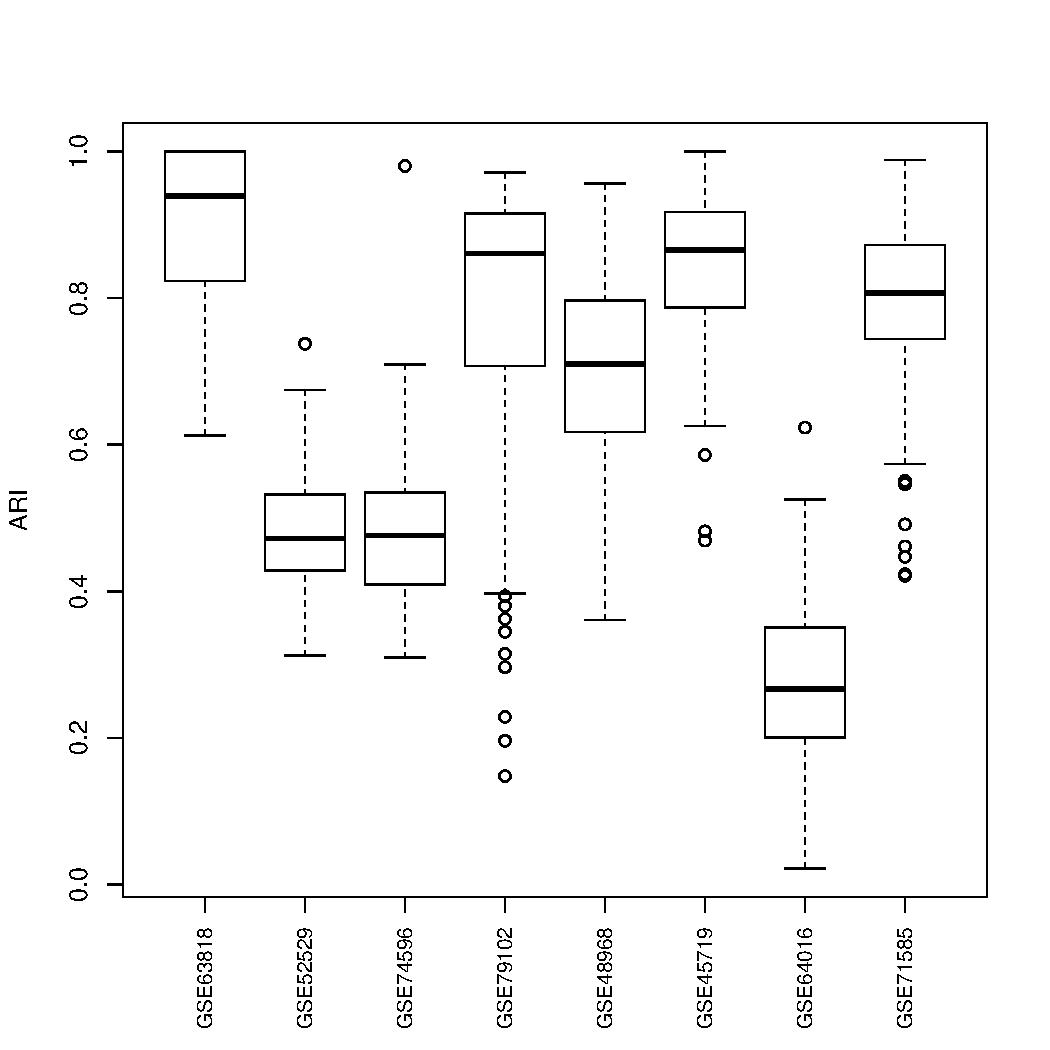
\includegraphics[scale = 0.7]{Figs/ARI.pdf}
 \caption{
 Adjusted rand indexes of randomly generated clustering to the one generated by the original distance matrix. 
 We investigate the variation of clustering given by random weighting through 8 datasets 
 and each dataset we are using 100 random distances.
}
  \label{fig:ARI}
\end{figure}

We plot the ARI(adjusted random index) between the randomly generated clustering to clustering under the original distance across eight datasets. Though the mean varies, the interquartile range is wide enough presenting a reasonable variation of our random weighting scheme.

We also check validity of random weighting on simulated dataset. 
We simulate one-dimensional data $X$ from a mixture of 5 normal distributions with different means and same variance ($\mu = (-3,-1,0,1,5), \sigma = 1$). 
We compare clustering results between random weighting and bayesian clustering using Dirichlet process as prior in terms of posterior probabilities that two elements belong to the same class given the whole data. 
We also compare accuracy of the two procedures by looking at the ARI comparing to true class label (supplementary Figure \ref{fig:simu}).  
We found that random weighting scheme tends to give better results than classical bayesian clustering.

\begin{figure}[h!]
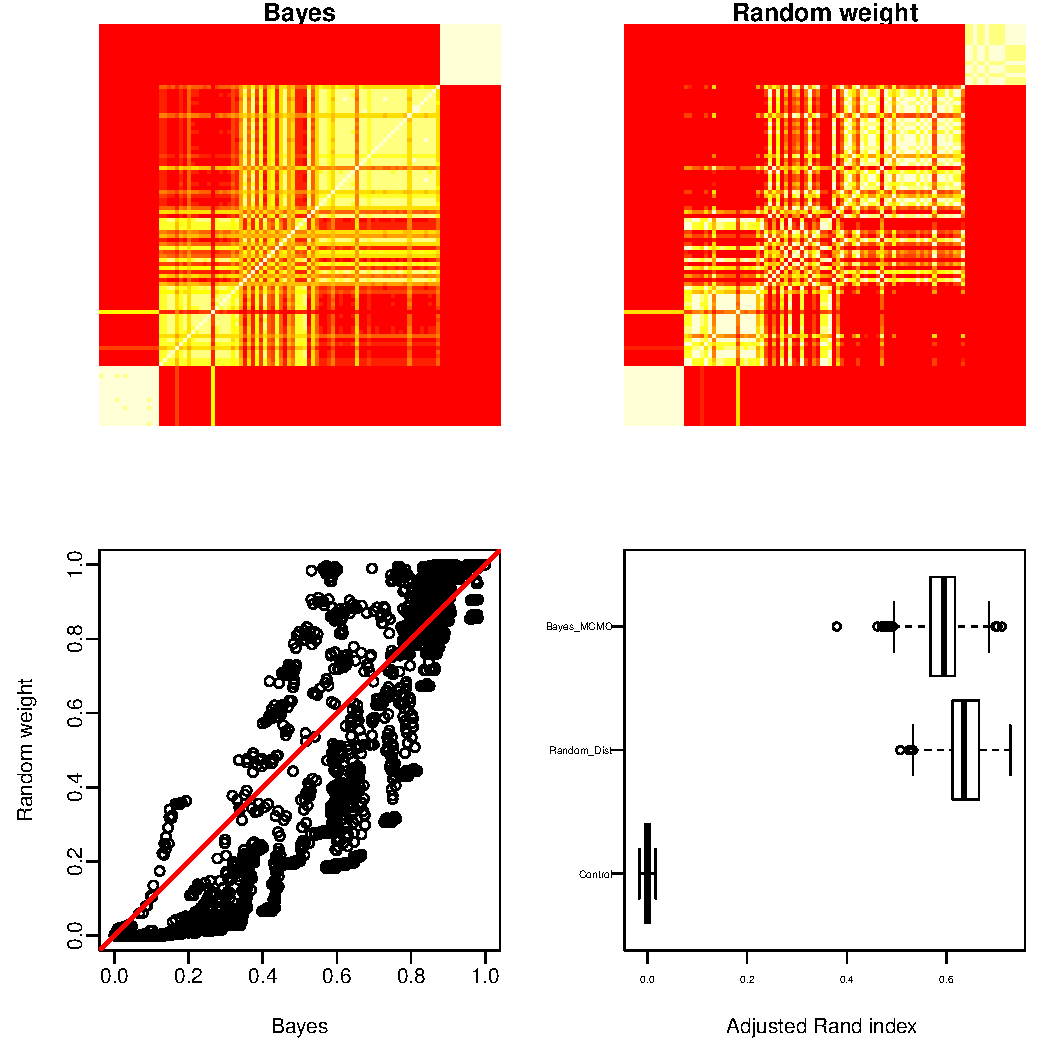
\includegraphics[scale = 1]{Figs/try7-g.pdf}
 \caption{comparison between random weighting scheme and bayesian clustering procedure in terms of posterior probabilities that two elements belong to the same class given the whole data and adjusted rand index comparing to the underlying true class label}
  \label{fig:simu}
\end{figure}



\subsubsection{Selecting $K$}

In this section, we gave the criterion to select $K$.

In order to determine the number of clusters and inspired by \verb validity defined in \cite{selK},
We consider a modified \verb validity = $\frac{\textbf{intra}}{\textbf{inter}}$.
where $\textbf{intra} = \frac{1}{N}\overset{K}{\underset{i = 1}{\Sigma}}\underset{x \in C_i}{\Sigma} ||x - z_i||^2$, 
$\textbf{inter} = mean( || z_i - z_j||^2), i,j = 1,2,...K$ and $z_i$ is the center(medoids) of cluster $i$. 
$\textbf{intra}$ is the average of distance of a point to its corresponding cluster center, which measures the compactness of clusters. 
$\textbf{inter}$ is the average distance of two cluster centers, which measures the separation between clusters.
Here, we made a small change, in original paper $\textbf{inter}$ was defined as minimum distance between medoids, 
we use average for the purpose of getting a smoother quantity. 
We want to have a small intra-cluster distance and a big inter-cluster distance, consequently we want to minimize the \verb validity.
From empirical study, we constantly observe a monotone decreasing relation between number of clusters and \verb validity. 
However this quantity stabilize when $K$ is sufficiently large. The stopping rule for searching $K$ is when $\texttt{validity}_{K}  < \epsilon$ is satisfied. We set the default value of  $\epsilon$ to be 1.  As we found DD analysis results to be most consistent with other scRNA method.



\subsection{Double Dirichlet Mixture}

In this section, we gave proofs for the properties and theorem for DDM in section 2.3 of main paper.

On the double Dirichlet masses, using notations in the main paper we have density functions:


\begin{eqnarray*}
p_\pi(\phi,\psi) =
         q_\pi( \Phi_\pi, \Psi_\pi  ) \, \prod_{b \in \pi}  \left[
         p( \tilde \phi_b ) p( \tilde \psi_b ) \right]
\end{eqnarray*}
with
\begin{eqnarray*}
q_\pi( \Phi_\pi, \Psi_\pi  )
= \frac{\Gamma(\sum_{b\in \pi} \beta_b)}{
 \prod_{b \in \pi} \Gamma( \beta_b )} \left[\prod_{b \in \pi} \Phi_b^{\beta_b-1} \right] \,
 1\left[ \Phi_\pi = \Psi_\pi \right]
\end{eqnarray*}
and
\begin{eqnarray*}
p( \tilde \phi_b ) =
\frac{ \Gamma( \sum_{k\in b} \alpha_k ) }{ \prod_{k\in b} \Gamma(\alpha_k) }
 \prod_{k \in b} \tilde \phi_k^{\alpha_k -1 },
\qquad
p( \tilde \psi_b )
=
\frac{ \Gamma( \sum_{k\in b} \alpha_k ) }{ \prod_{k\in b} \Gamma(\alpha_k) }
\prod_{k \in b} \tilde \psi_k^{\alpha_k -1 }.
\end{eqnarray*}

Those computing units will serve as key components for proofing property 1 $\sim$ 6 in section 2.3

Proof of property 1
\begin{proof}
When $\phi$ and $\psi$ only satisfy the coarsest constrants: $\sum_{i = 1}^K \phi_i = \sum_{i = 1}^K \psi_i = 1$. $\phi$ and $\psi$ are independently Dirichlet distributed.
When $\phi$ and $\psi$ satisfy finer constraints, $P(\phi | \psi ) \neq P(\phi)$ as there is some subsets $b \neq \pi$ such that $\sum_{i\in b} \phi = \sum_{i \in b} \psi$. So $\phi$ and $\psi$ are dependent
\end{proof}

Proof of property 2
\begin{proof}
$E_{\pi}(\phi_k) = E_{\pi}(\phi_k | \Phi_b) E_{\Phi}(\Phi_b) = E_{\tilde{\phi}_b}(\tilde{\phi}_k)E_{\Phi}(\Phi_b)$ where $b$ is the block containing subtype index $k$.As $\tilde{\phi}_b \sim  \text{Dirichlet}_{N(b)}[ \alpha_b^1 ]$ and  $\Phi_\pi  \sim \text{Dirichlet}_{N(\pi)}[   \beta_\pi   ] $
We have $E_{\tilde{\phi}_b}(\tilde{\phi}_k) =  \frac{ \alpha^1_k }{ \sum_{k' \in b} \alpha^1_{k'} } $ and $E_{\Phi}(\Phi_b) = \frac{ \beta_b }{ \sum_{b' \in \pi} \beta_{b'} } $. Similarly we could proof the case for $E_{\pi}(\psi_k)$
\end{proof}

Proof of property 3
\begin{proof}
$t^1 / t_{\pi}^1$ is independent with $t^2 / t_{\pi}^2$ conditioning on $t_\pi^1$ and $t_\pi^2$ by the Neutrality property of Dirichlet distribution
\end{proof}

Proof of property 4
\begin{proof}
For $j = 1,2$,
let $T_b^j$ be the vector of $t_k^j$ such that $k \in b$. Recall $t_b^j = \sum_{k \in b} t_k^j$.
Without loss of generality, we consider the case condition $j = 1$.\\
At the support of $p_\pi$, for different blocks, $T_b^1 | \tilde \phi_b$ are mutually independent. Then we have factorization:
\begin{eqnarray*}
p_\pi(t^1 | t_\pi^1, y) = \prod_{b\in \pi}(p(T_b^1 | t_b^1,y) )
\end{eqnarray*}
and right hand side prior predictive function can be obtained via integral out $ \tilde{\phi}_b$ given the prior $\text{Dirichlet} [ \alpha_b^1]$ and  $p(T_b^1  | \tilde{\phi}_b)$ is multinomial($\tilde{\phi}_b)$ distributed.
\begin{align*}
p(T_b^1  | t_b^1,y) &= \int_{\tilde{\phi}_b} p(T_b^1  | \tilde{\phi}_b) p(\tilde{\phi}_b) d\tilde{\phi}_b\\
                                      &= \left\{\left[ \frac{ \Gamma(t^j_b +1 ) }{\prod_{k \in b} \Gamma( t^j_k + 1 ) }\right]
\left[ \frac{\Gamma( \sum_{k \in b} \alpha_k^j )}{
		\prod_{k\in b} \Gamma( \alpha_k^j ) } \right] 
       \left[        \frac{ \prod_{k \in b} \Gamma(\alpha_k^j + t^j_k)  }{
		\Gamma(t^j_b + \sum_{k\in b} \alpha_k^j ) )}\right]\right\}
\end{align*}
\end{proof}

Proof of property 5
\begin{proof}
$t_\pi^1$ and $t_\pi^2$ given the condition label $y$ are independent identical distributed. $t_\pi^1 |\Phi \sim$ multinomial$(\Phi)$
\begin{align*}
p_\pi(t^1_{\pi},t^2_{\pi}| y) &= \int_\Phi p(t_\pi^1 | \Phi) p(t_\pi^2 | \Phi) p(\Phi) d\Phi \\
&= \left[ \frac{ \Gamma(n_1+1) \Gamma(n_2+1) }{ \prod_{b \in \pi} \Gamma(t^1_b+1) 
   \Gamma( t^2_b + 1 )} \right] 
\left[ \frac{\Gamma( \sum_{b \in \pi} \beta_b  )}{
   \prod_{b \in \pi} \Gamma(\beta_b )} \right] 
 \left[ \frac{ \prod_{b \in \pi} \Gamma( \beta_b + t^1_b + t^2_b )}{
	\Gamma( n_1 + n_2 + \sum_{b \in \pi} \beta_b  )} \right].
\end{align*}
As prior of $\Phi \text{ is Dirchlet}[ \beta ] \text{ and } n_j = \sum_{b \in \pi} t_b^j \text{ for } j = 1,2$
\end{proof}


To prove property 6, we need a lemma of dimensionality of the intersection of two $A_\pi$s 
\begin{lemma}
If $\pi_2$ is not refinement of $\pi_1$ then $A_{\pi_1} \cap A_{\pi_2}$ is a lower dimensional subset of $A_{\pi_2}$
\end{lemma}

Proof of lemma 1
\begin{proof}
Let $V$ denote the orthogonal space of $\phi - \psi$, when $(\phi,\psi)\in A_{\pi_1} \cap A_{\pi_2}$, and $\text{dim}(A_{\pi_1} \cap A_{\pi_2}) = \text{dim}(\phi - \psi) + \text{dim}(\psi) = 2K - \text{dim}(V) - 1$. Also let $\pi_1 = \{b_1^1,...,b_s^1\}, \pi_2 = \{b_1^2,...,b_t^2\}$. The corresponding vectors are $v_1^1,...,v_s^1$ and $v_1^2,...,v_t^2$. We claim there must be a $b_i^1\in \pi$ whose corresponding $v_i^1$ is linear independent with $v_1^2,...,v_t^2$. If not, for every $v_i^1$ there exists $\alpha_1^i,...,\alpha_t^i$ such that 
\[
v_i^1 = \sum_{j = 1}^t \alpha_j^i v_j^2 \quad\quad\quad(*)
\]
If $b_j^2 \cap b_i^1 \neq \emptyset$, then multiply $v_j^2$ on both sides of (*), we obtain $v_i^1 * v_j^2 = \alpha_j^i (v_j^2)^2$, as $v_j^2$ are orthogonal vectors, and $v_i^1 * v_j^2 > 0$ implies $\alpha_j^i > 0$. Consider $x = f(b_j^2\setminus b_i^1)$, we have $x*v_i^1 = 0$ and we multiply $x$ on both sides of (*) to obtain $\alpha_j^i v_j^2*x = 0$, thus x must be zero vector and $b_j^2\setminus b_i^1= \emptyset$, which implies $b_j^2 \subset b_i^1$. That is to say when $b_j^2 \cap b_i^1 \neq \emptyset$, $b_j^2$ must be subset of $b_i^1$. So $b_i^1$ is union of some blocks in $\pi_2$. Which implies $\pi_2$ is refinement of $\pi_1$, contradiction.\\
Consequently there exists $b\in\pi_1$ with $v(b)$ linear independent with $v(b'), b'\in\pi_2$. $\text{dim}(V)$ is at least $N(\pi_2) + 1, \dim(A_{\pi_1} \cap A_{\pi_2}) < \text{dim}(A_{\pi_2})$
\end{proof}

Proof of property 6
\begin{proof}
For a $\pi$, $P(A_\pi, | y, z) = \underset{\tilde \pi \in \Pi}{\sum} \int_{A_{\pi}} \omega_{\tilde \pi}^{\text{post}} d\phi d\psi$, notice the support of $\omega_{\tilde \pi}^{\text{post}$ is $A_{\tilde \pi}$. 
By lemma 1, we know if $\tilde \pi$ does not refine $\pi$, then $\int_{A_{\pi}} \omega_{\tilde \pi}^{\text{post}} d\phi d\psi$ is an integral on lower dimension set and vanish. if $\tilde \pi$ refines $\pi$, then 
$\int_{A_{\pi}} \omega_{\tilde \pi}^{\text{post}} d\phi d\psi = $\int_{A_{\tilde \pi}} \omega_{\tilde \pi}^{\text{post}} d\phi d\psi = \omega_{\tilde \pi}^{\text{post}}$. We have $P(A_\pi, | y, z) = \underset{\tilde \pi \in \Pi}{\sum} \omega_{\tilde \pi}^{\text{post}} 1[\tilde \pi \text{ refines } \pi ]$
\end{proof}

Proof of theorem 3
\begin{proof}
%$p_\pi ( t^1 | t_\pi^1, y) p_\pi ( t^2 | t_\pi^2 , y) p_\pi ( t_\pi^1, t_\pi^2 | y )$
Recall the DDM prior: $p(\phi,\psi) = \sum_{\pi \in \Pi} p_\pi(\phi,\psi)$. 
By bayes' rule we know $p(\phi,\psi | y,z) \propto p(\phi,\psi, y, z) = \sum_{\pi \in \Pi}  p(y, z | \phi,\psi) p_\pi(\phi,\psi)\omega_\pi$
and we use the 1-1 map from $(\phi,\psi)$ to $(\tilde \phi, \tilde \psi, \Phi)$ to get
\begin{eqnarray*}
p(y, z | \phi,\psi) p_\pi(\phi,\psi) = p(y, z | \tilde{\phi} , \tilde{\psi}, \Phi_\pi) p(\tilde{\phi}) p (\tilde{\psi}) p(\Phi_\pi)
\end{eqnarray*}
when $(\phi,\psi) \in A_\pi$.
Let us denote right hand side of the above equation as $U_\pi$, then
\begin{eqnarray*}
U_\pi = \omega_\pi A_1 A_2 A_3\prod_{k = 1}^K (\tilde{ \phi }_k)^{t_k^1 + \alpha_k^1} (\tilde{ \psi }_k)^{t_k^2 + \alpha_k^2}   \prod_{b \in \pi} (\Phi_b)^{t_b^1 + t_b^2 + \beta_b}
\end{eqnarray*}
Where $A_1$ is the product of normalizing terms from multinomial distribution of $z^1$ and $z^2$, $A_1 =  \frac{\Gamma(n_1 + 1)\Gamma(n_2 + 1)}{\prod_{j = 1}^2\prod_{k = 1}^K \Gamma(t_k^j + 1) } $\\
$A_2$ is the product of normalizing terms from Dirichlet distribution of $\tilde{\phi}$ and $\tilde{\psi}$,
$A_2 = \frac{ \Gamma( \sum_{k = 1}^K \alpha_k^1 + 1)  \Gamma( \sum_{k = 1}^K \alpha_k^2 + 1)}{ \prod_{j = 1}^2 \prod_{k = 1}^2 \Gamma(\alpha_k^j + 1)}$\\
$A_3$ is the normalizing term from Dirichle distribution of $\Phi_\pi$, $A_3 = \frac{\Gamma(\sum_{b \in \pi } \beta_b + 1)}{\prod_{b\in \pi} \Gamma(\beta_b + 1)}$\\
Looking at the indexes of $\tilde \phi, \tilde \psi \text{ and } \Phi$, we can decompose $U_\pi$ as product of three Dirichlet densities with a normalizing term. 
Namely $U_\pi = C_\pi * f_1 f_2 f_3$, where
$f_1 \sim \text{Dirichlet}[\alpha^1 + t^1]$, $f_2 \sim \text{Dirichlet}[\alpha^2 + t^2]$ and $f_3 \sim \text{Dirichlet}[\beta + t^1 + t^2]$.
Considering the normalizing factors for densities $f_1,f_2$ and $f_3$, and multiplying them with $A_1, A_2$ and $A_3$. 
We have the $C_\pi =  p_\pi(t^1 | t^1_{\pi},y)\, p_\pi(t^2|  t^2_{\pi},y )
 \, p_\pi( t^1_{\pi}, t^2_{\pi} | y ) \omega_\pi$. \\
 Consequently, we have 
 \begin{eqnarray*}
 (\phi,\psi)|y,z  \sim {\mbox {\rm DDM}}\left[ \omega^{\rm post}=(\omega^{\rm post}_\pi), \alpha^1 + t^1, \alpha^2 + t^2  \right] \text{ and } \omega^{\rm post}_\pi \propto 
 p_\pi(t^1 | t^1_{\pi},y)\, p_\pi(t^2|  t^2_{\pi},y )
 \, p_\pi( t^1_{\pi}, t^2_{\pi} | y ) \, \omega_\pi.
 \end{eqnarray*}
 Notice in DDM, we restricted $\beta = \alpha^1 + \alpha^2$.

\end{proof}


\section{Numerical Experiments}

\subsection{Synthetic Data}
In this section, we use pca plots to show the subtle changes underlying each subtypes of simulated data and 
we demonstrate consistency of estimated distributional changes based on \texttt{scDDboost} and Wasserstein distance.
Finally, roc curve illustrates that \textt{scDDboost} having a good operating characteristic. 


We first look at the pca plots of the simulated data (supplementary figure \ref{fig:pca1}, \ref{fig:pca2}, \ref{fig:pca3}).
For $K = 7 \text{ and } 12$, each scenario there were some subtypes nested in the 2d PCA projection. 
The distributional change of transcripts becomes difficult to detect. 
\texttt{scDDboost} benefits from the compositional structure and is more sensitive to those subtle changes.

\begin{figure}[h!]
  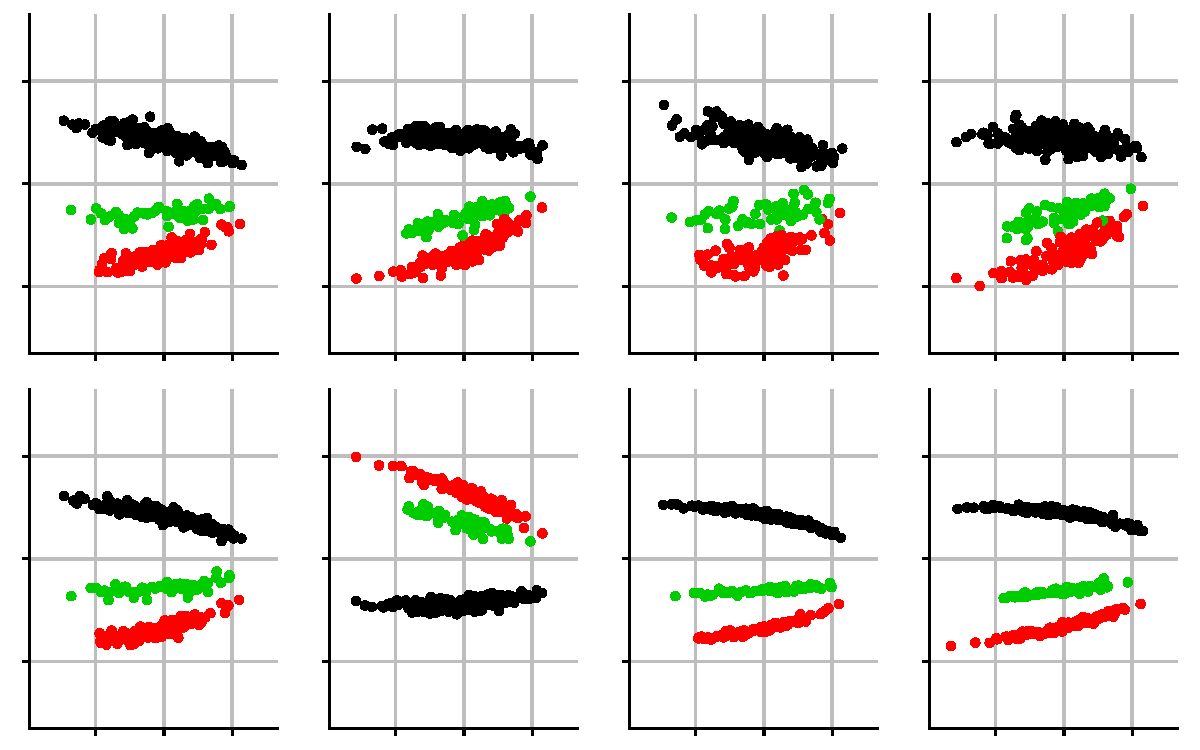
\includegraphics[ width = 0.8\textwidth]{Figs/pca3.pdf}
  \caption{first two principal components of transcripts under different parameters for simulated data. Different parameters resulted in different degree of separation of subtypes. We have 4 different settings for hyper-parameters of simulation, each setting has 2 replicates K = 3}
  \label{fig:pca1}
\end{figure}


\begin{figure}[h!]
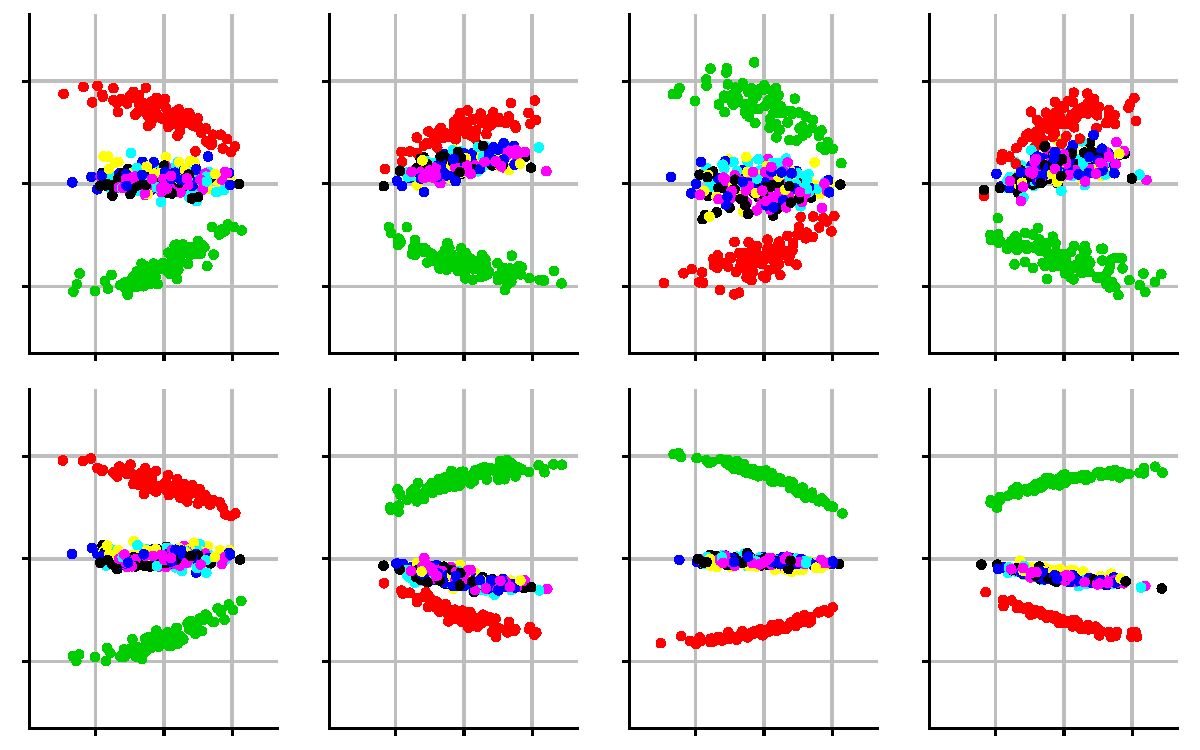
\includegraphics[ width = 0.8\textwidth]{Figs/pca7.pdf}
\caption{K = 7}
\label{fig:pca2}
\end{figure}

\begin{figure}[h!]
  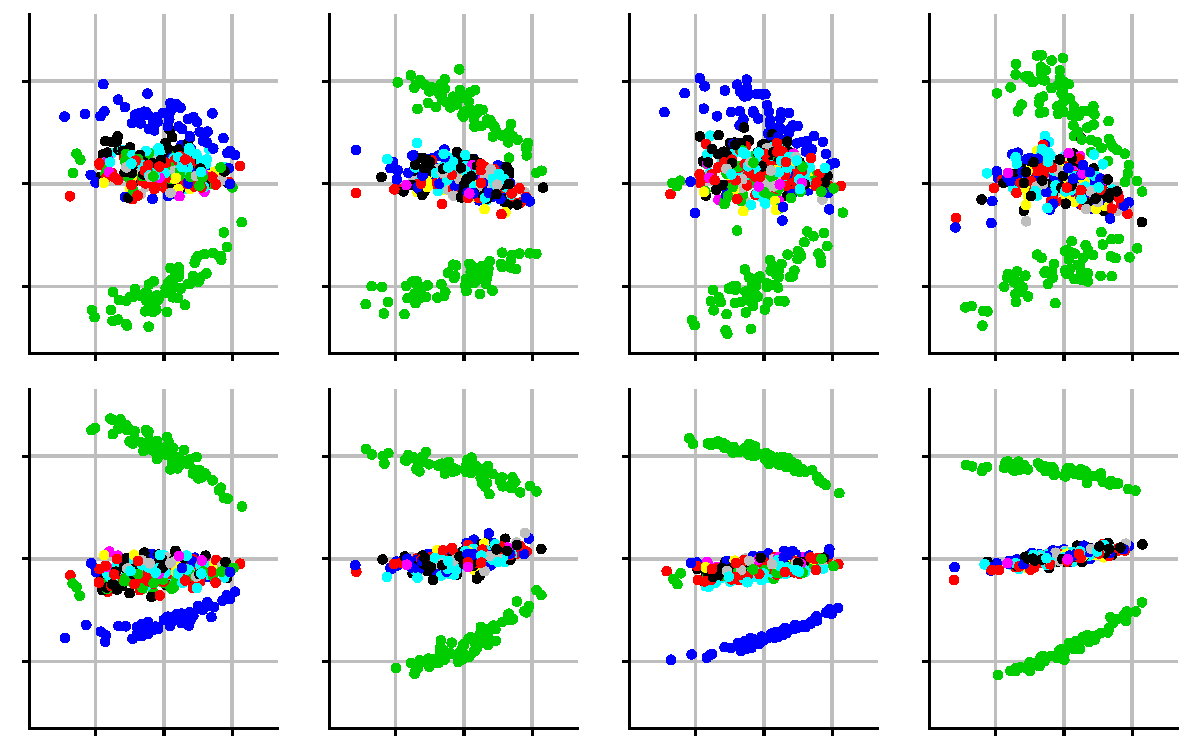
\includegraphics[ width = 0.8\textwidth]{Figs/pca12.pdf}
  \caption{K = 12}
  \label{fig:pca3}
  \end{figure}
  
  
We observed consistent measurements of distributional change based on \texttt{scDDboost} and Wasserstein distance between the empirical distribution of transcripts.(supplementary figure \ref{fig:simu_wad})
Lower probabilities of equivalent distributed are associated with bigger distances.
\begin{figure}[h!]
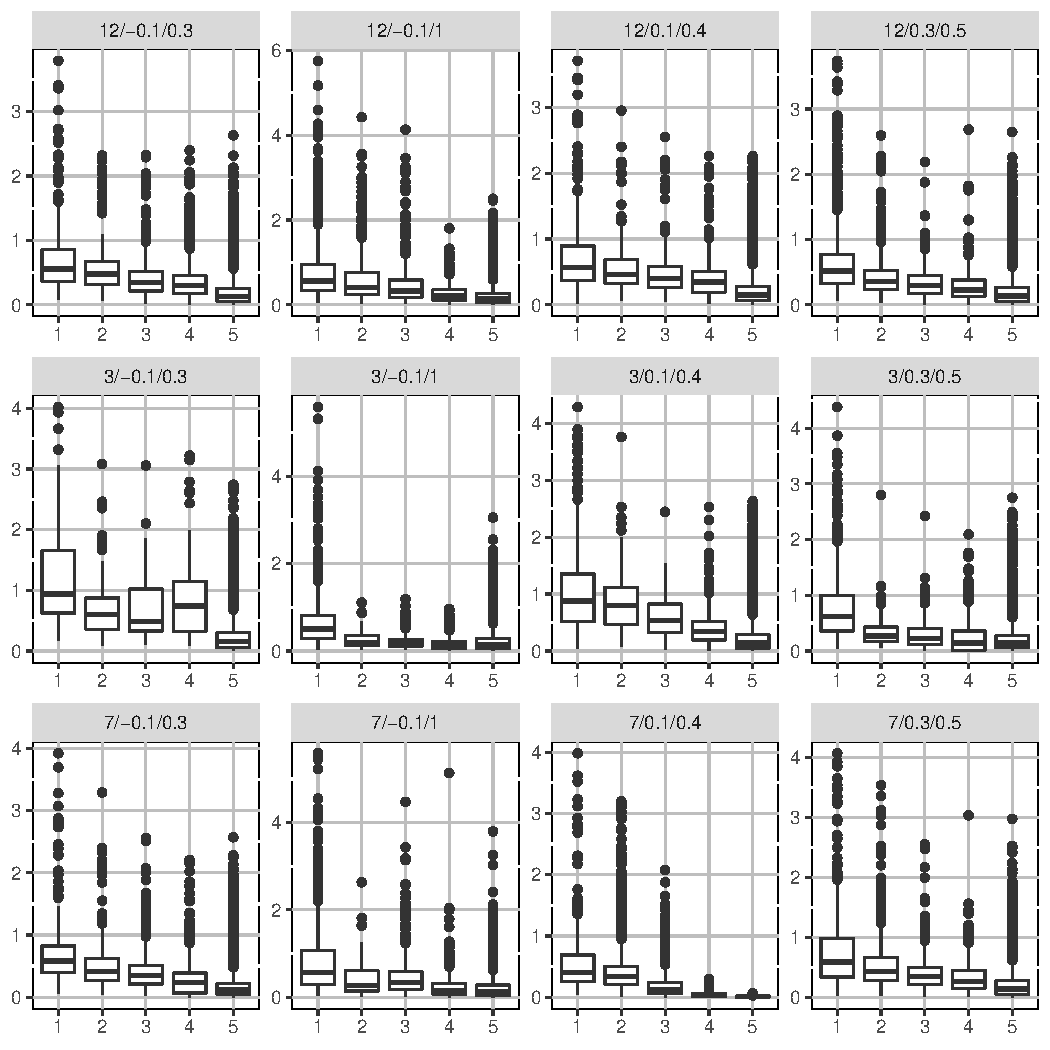
\includegraphics[width = 0.6\textwidth]{Figs/simu_wadist.pdf}
\caption{$P(ED_g|X,y)$ given by scDDboost versus empirical Wasserstein distance. 
Genes associated with boxes from left to right having $P(ED_g|X,y)$ range from 0 - 0.2, 0.2 - 0.4, 0.4 - 0.6, 0.6 - 0.8, 0.8 - 1. For the simulation cases}
 \label{fig:simu_wad}
\end{figure}


  
  
\clearpage

We also have roc curve for the simulated data, each sub-figure is averaged over two replicates under the same parameters setting. scDDboost tends to outperform other methods (supplementary figure \ref{fig:roc})
\begin{figure}[h!]
  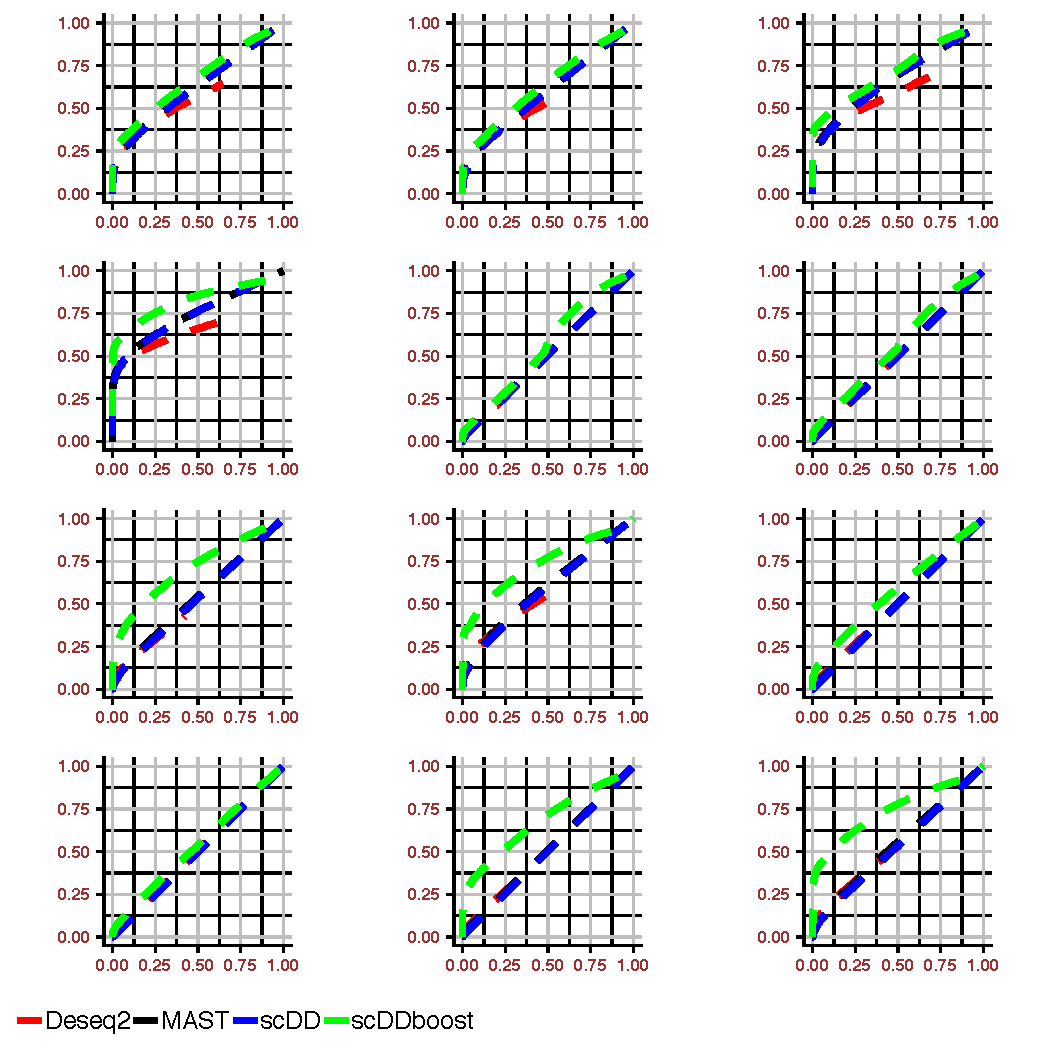
\includegraphics[ width = 0.8\textwidth]{Figs/Roc_supp.pdf}
  \caption{Roc curve of the 12 simulation settings, under each setting, TPR and FPR are averaged over two replicates, generally we found scDDboost perform better than other methods}
  \label{fig:roc}
\end{figure}



\clearpage

\subsection{Empirical Study}

In this section, we gave details of the empirical datasets and also demonstrate consistency to Wasserstein distance on one dataset (FUCCI).


\noindent
{\bf Data sets} details for the datasets used in the empirical studies of the main paper and the estimated number of subtypes $K$ (supplementary table \ref{table:1})



\begin{table}[h!]
\small
\centering
\begin{tabular}{ |p{2cm}|p{5cm}|p{2cm}|p{2cm}|p{2cm}|p{1cm}|}
\hline
 Data set & Conditions & Number of cells/condition & Organism  & Ref & K\\ \hline \hline
GSE94383 & 0 min unstim vs 75min stim & 186,145 & human & \citep{Lane} & 9\\ \hline
GSE48968-GPL13112 & BMDC (2h LPS stimulation) vs 6h LPS & 96,96 & mouse & \citep{Shalek} & 4\\ \hline
%GSE60749-GPL13112 & serum + LIF vs  2i + LIF & 90,94 & mouse & \citep{Kumar} & 5\\ \hline
GSE52529 & T0 vs T72 & 69,74 & human & \citep{Trapnell} & 7\\ \hline
GSE74596 & NKT1 vs NTK2 & 46,68 & mouse & \citep{Engel} & 7\\ \hline
EMTAB2805 & G1 vs G2M & 95,96 & mouse & \citep{EMTAB} & 6\\ \hline
GSE71585-GPL13112 &Gad2tdTpositive vs Cux2tdTnegative  & 80,140 & mouse & \citep{Tasic} & 4\\ \hline
GSE64016 & G1 vs G2 & 91,76 & human & \citep{oscope} & 6\\ \hline
GSE79102 & patient1 vs patient2 & 51, 89 & human & \cite{sc3} & 4\\ \hline
GSE45719 & 16-cell stage blastomere vs mid blastocyst cell & 50, 60 & mouse & \citep{Deng193} & 4\\ \hline
GSE63818 & Primordial Germ Cells, develop- mental stage: 7 week gestation vs Somatic Cells, developmental stage: 7 week gestation & 40,26 & mouse & \citep{Guo} & 6\\ \hline
GSE75748 & DEC vs EC & 64, 64 & human & \citep{chu} & 5\\ \hline
GSE84465 & neoplastic cells vs non-neoplastic cells & 1000, 1000 & human & \citep{Darmanis} & 9\\ \hline
\end{tabular}
\captionof{table}{datasets used for comparisons of DD analysis under different methods}
\label{table:1}
\end{table}

The largest dataset we tried is GSE84465, we randomly sampled 1000 cells from each condition. The reason is that we in total have 3500 cells, it takes more time and memories to compute if we consider all the samples and 
1000 cells each condition would be enough to represent the heterogeneity. We found \texttt{DESeq} identified significant smaller number of positives than others. It is intuitive that we are more likely to encounter subtle changes
when we have large samples. Only consider mean shifts would have limited power. For other datasets we use all the cells within that condition under same batch.

We also observed consistent distributional change measurements by \texttt{scDDboost} and Wasserstein distance between the empirical distribution of transcripts .
(supplementary Figure \ref{fig:wad})

\begin{figure}[h!]
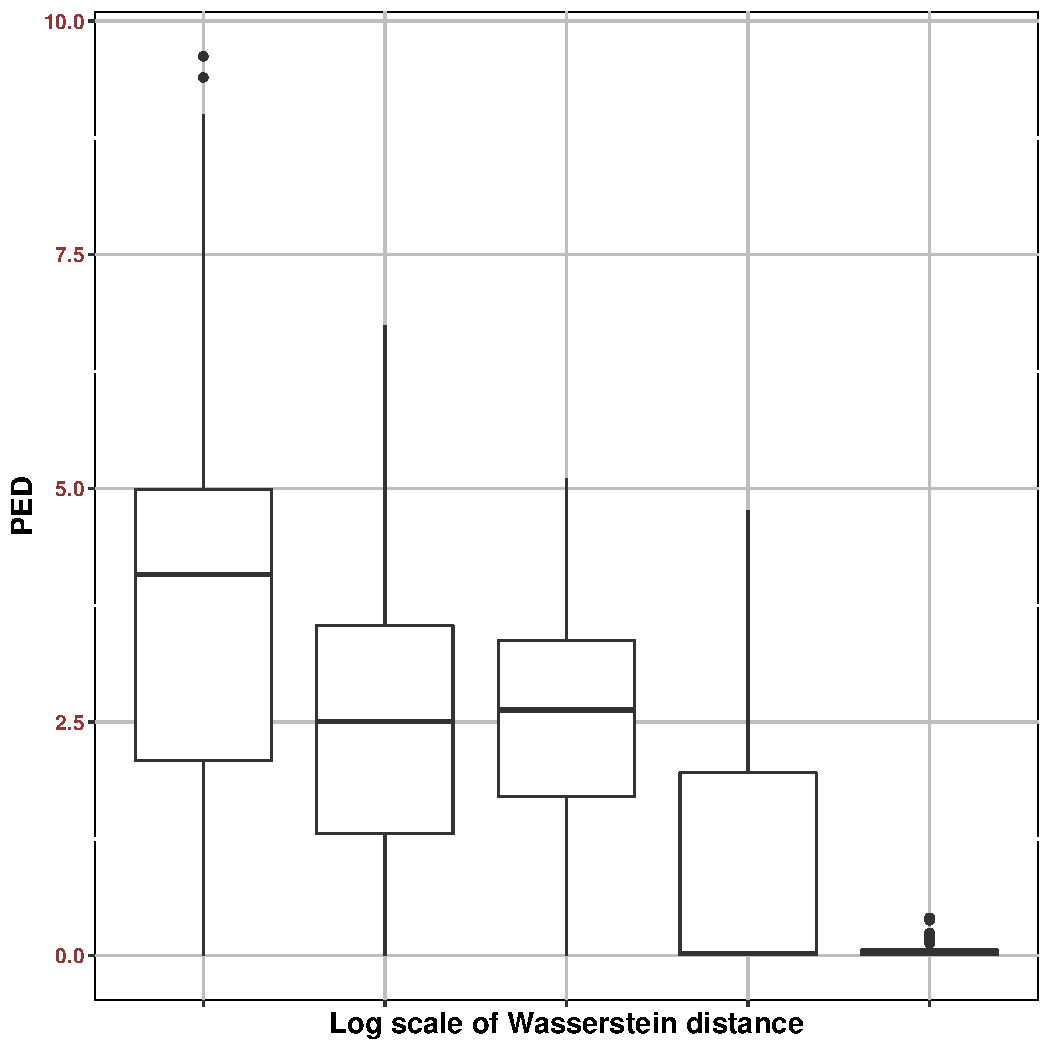
\includegraphics[width = 0.4\textwidth]{Figs/Fucci_wadist.pdf}
\caption{$P(ED_g|X,y)$ given by scDDboost versus empirical Wasserstein distance. 
Genes associated with boxes from left to right having $P(ED_g|X,y)$ range from 0 - 0.2, 0.2 - 0.4, 0.4 - 0.6, 0.6 - 0.8, 0.8 - 1, data used: FUCCI}
 \label{fig:wad}
\end{figure}






Datasets used for generating the Null cases (supplementary table \ref{table:2})

\begin{table}[h!]
\footnotesize
\centering
\begin{tabular}{ |p{3cm}|p{5cm}|p{3cm}|p{2cm}|}
\hline
 Data set & Conditions & Number of cells/condition & Organism \\
\hline
\hline
GSE63818null & 7 week gestation  & 20,20 &mouse \\
\hline
GSE75748null & DEC & 32, 32 & human\\
\hline
GSE94383null & T0 & 93, 93 & human \\
\hline
GSE48968-GPL13112null & BMDC (2h LPS stimulation) & 48,48 & mouse \\
%\hline
% GSE60749-GPL13112null & v6.5 mouse embryonic stem cells, culture conditions: 2i+LIF & 45,45 & mouse \\
 \hline
 GSE74596null & NKT1 & 23,23 & mouse\\
 \hline
 EMTAB2805null & G1 & 48,48 & mouse\\
 \hline
GSE71585-GPL13112null &Gad2tdTpositive  & 40,40 & mouse \\
\hline
GSE64016null & G1 & 46,45 & human \\
\hline
GSE79102null & patient1 & 26, 25 & human\\
\hline
\end{tabular}
\captionof{table}{datasets used for null cases, as cells are coming from same biological condition, there should not be any differential distributed genes, any positive call is false positive}
\label{table:2}
\end{table}

\clearpage

\subsection{Robustness}

In this section, we demonstrate change of PDD under different $K$ and the robustness we gain through random weighting. We also gave a warning that using arbitrarily large $K$ will inflate FDR. 

Number of subtypes $K$ is a crucial factor controlling the accuracy of our modeling. 
Too small $K$ may end up in an underfit such that cells within same subtype can still be very different,
mean expression change among subtypes is incapable to capture the distribution change for some genes and consequently reducing the power of \textsc{scDDboost}.
Too big $K$ may end up in an overfit such that two subtypes can be very similar, given we have fixed number of samples (cells), allowing more clusters will introduce may patterns (both for mean expression change and proportion change) to infer. Also notice the limitation of DDM model (see section 4), overestimating $K$ in \textsc{scDDboost} may losing FDR control (supplementary Figure \ref{fig:lfdr}).

From our empirical experience, 
it would be sufficient to capture the heterogeneity underlying cells with number of clusters less than 10(supplementary Table 1).  
And we generally obtain stable validity score and PDD simultaneously (supplementary Figure \ref{fig:rwk})
We demonstrate the change of PDD given different $K$ at data GSE75748. When we increase $K$, the variance of the differential term $\text{PDD}_{K + 1} - \text{PDD}_K$ keeps decreasing and PDD keeps increasing. Our selection criterion (K = 5) happens to choose $K$ such that  change between $\text{PDD}_{K + 1}$ and $\text{PDD}_K$ is small while not inflating PDD.
\begin{figure}[h]
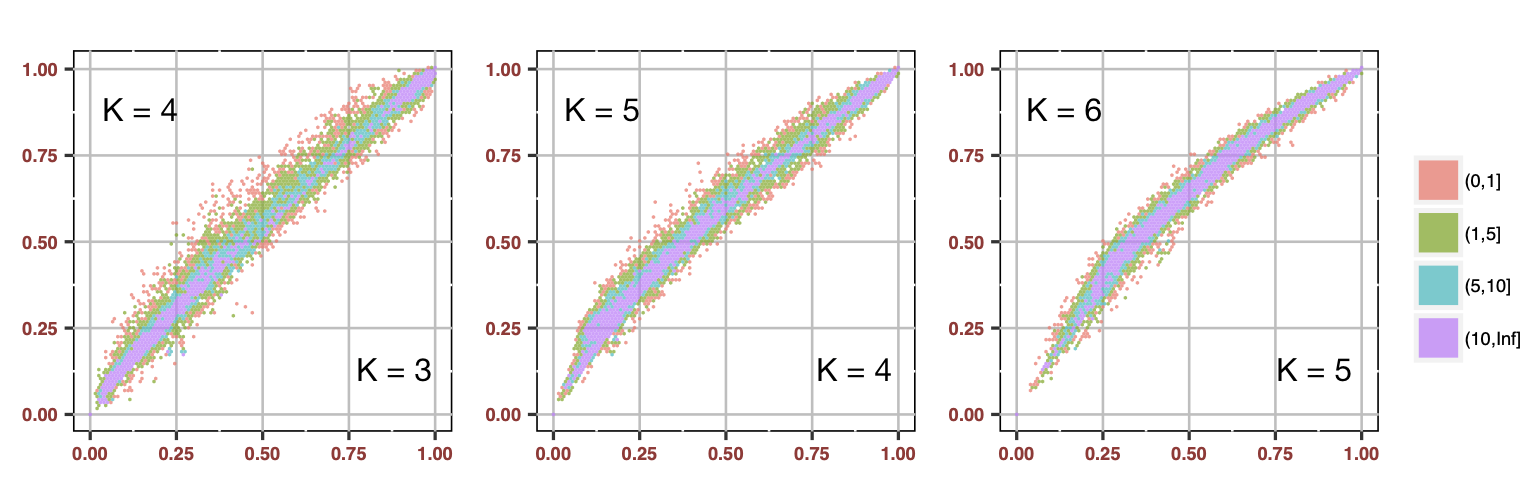
\includegraphics[width = 1\textwidth]{Figs/Kchange.png}
\caption{PDD change under different number of subtypes $K$, dataset used DEC-EC, our rule for selecting $K$ tends also to make PDD stabilize}
\label{fig:rwk}
\end{figure}

The random weighting scheme help us obtain robust PDD. 
\begin{figure}[h]
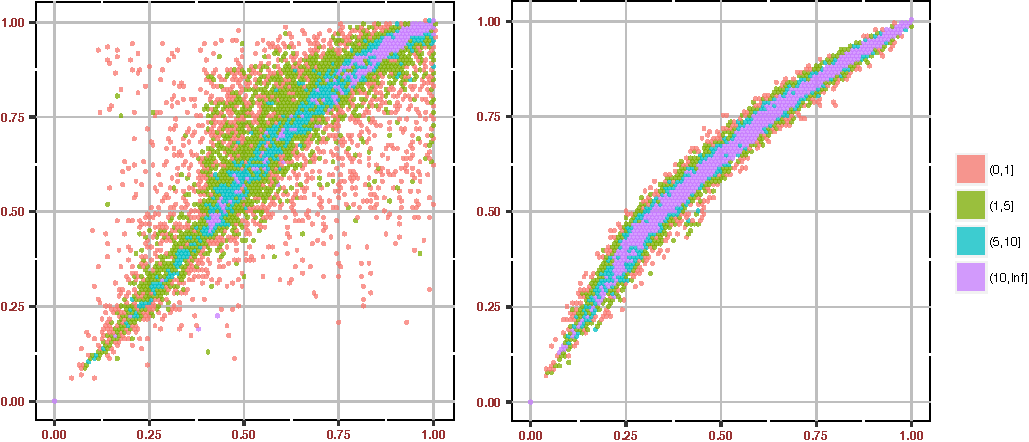
\includegraphics[width = 0.7\textwidth]{Figs/rw.pdf}
\caption{DEC-EC, PDD under K = 5 vs. K = 6, left panel is without the randomized distance and right panel is with randomized distance. We increase robustness of our methods through random weighting}
\end{figure}

scDDboost may lose FDR control if we keep increasing $K$.
\begin{figure}[h]
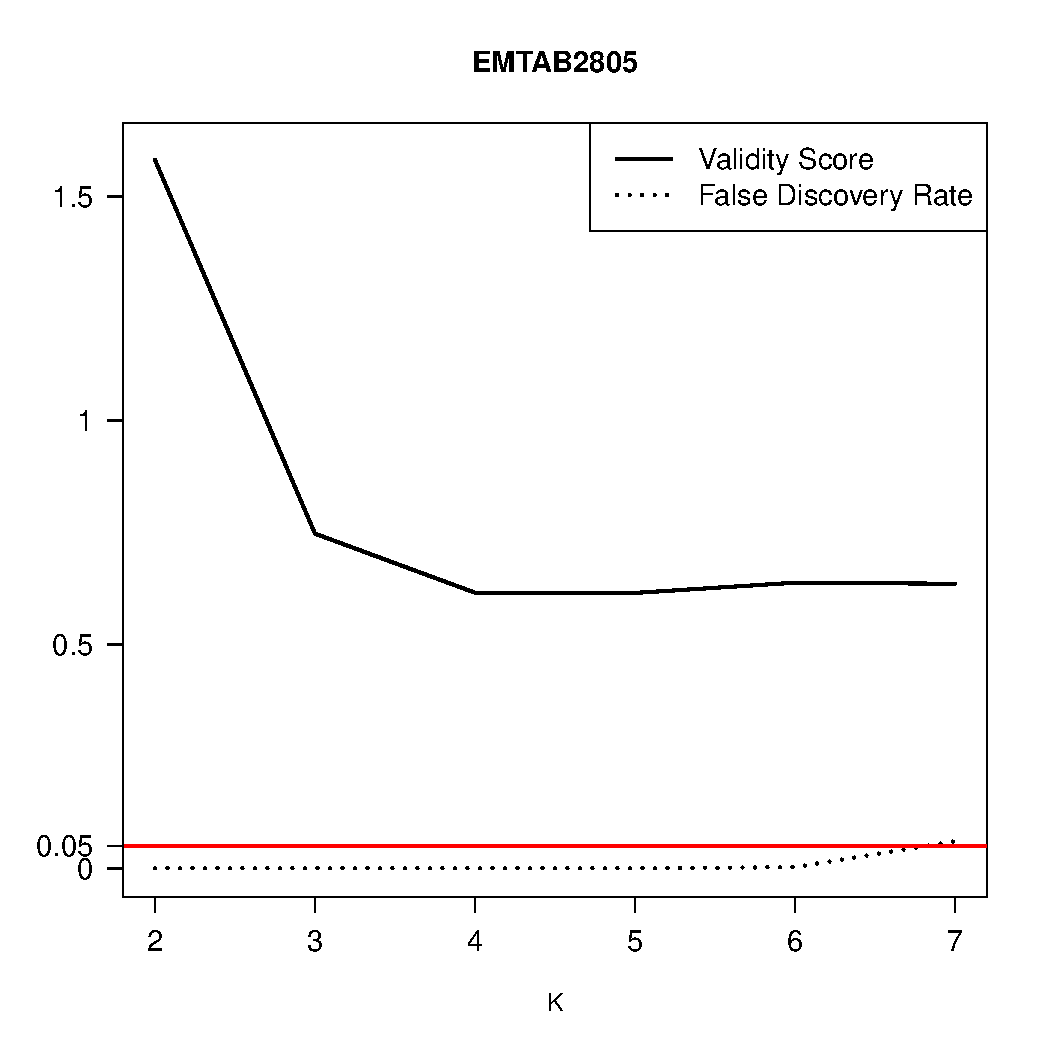
\includegraphics[width = 0.5\textwidth]{Figs/breakFDR.pdf}
 \caption{under NULL case, using dataset EMTAB2805, when using too big $K$ we may lose FDR control (black dashed line shows proportion of false positive identified by scDDboost under 0.05 threshold, while validity score did not vary too much after $K$ is
 greater than 2 }
  \label{fig:lfdr}
\end{figure}

\clearpage

%\subsection{Bursting parameters}

%***on the method estimated p-value, update later***

%D3E\citep{ref:d3e} is a distributional method that can identify bursting parameters of transcripts. Rate of promoter activation, rate of promoter inactivation and the rate of transcription when the promoter is in the active state are estimated by D3E.  We investigate DD genes identified by scDDboost and their change of those three parameters on dataset GSE71585\\

%\begin{figure}[H]
%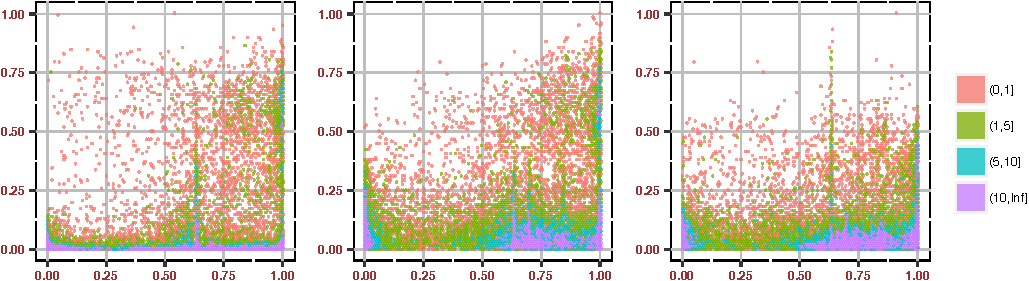
\includegraphics[width = 1\textwidth]{Figs/d3eplot.pdf}
%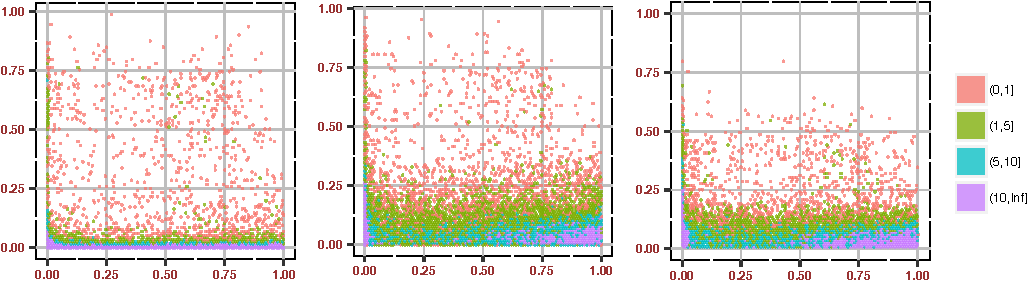
\includegraphics[width = 1\textwidth]{Figs/d3eplotdes.pdf}
%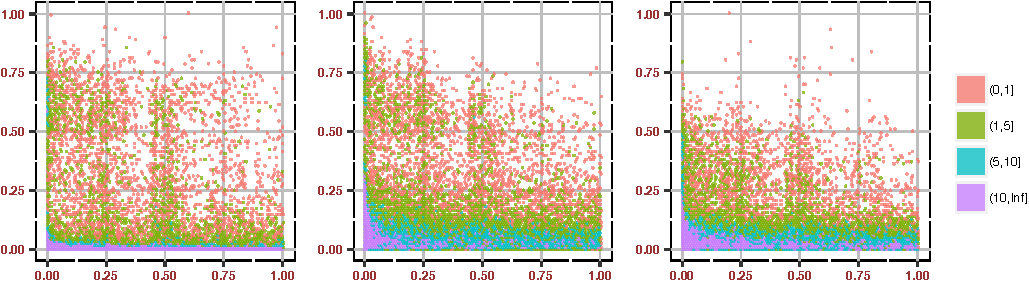
\includegraphics[width = 1\textwidth]{Figs/d3eplotmast.pdf}
%\includegraphics[width = 1\textwidth]{Figs/d3eplotscdd.pdf}
%\caption{D3E method will estimate 3 bursting parameters probability of a gene being on (\textbf{a}) and off (\textbf{b}) and the expression rate when the gene expression is on (\textbf{c}), we plot the hexbin plot of probability of a gene being DD under out method v.s. the absolute value of log fold change of \textbf{a} , \textbf{b} and \textbf{c}  across the two conditions accordingly. The log fold change is scaled by dividing the largest log fold change so that ends up in a value between 0 and 1 Here we use the GSE71585 data }
%\end{figure}



%\begin{figure}[h!]
%\vspace{-\parskip}
%\minipage{0.33\textwidth}
%  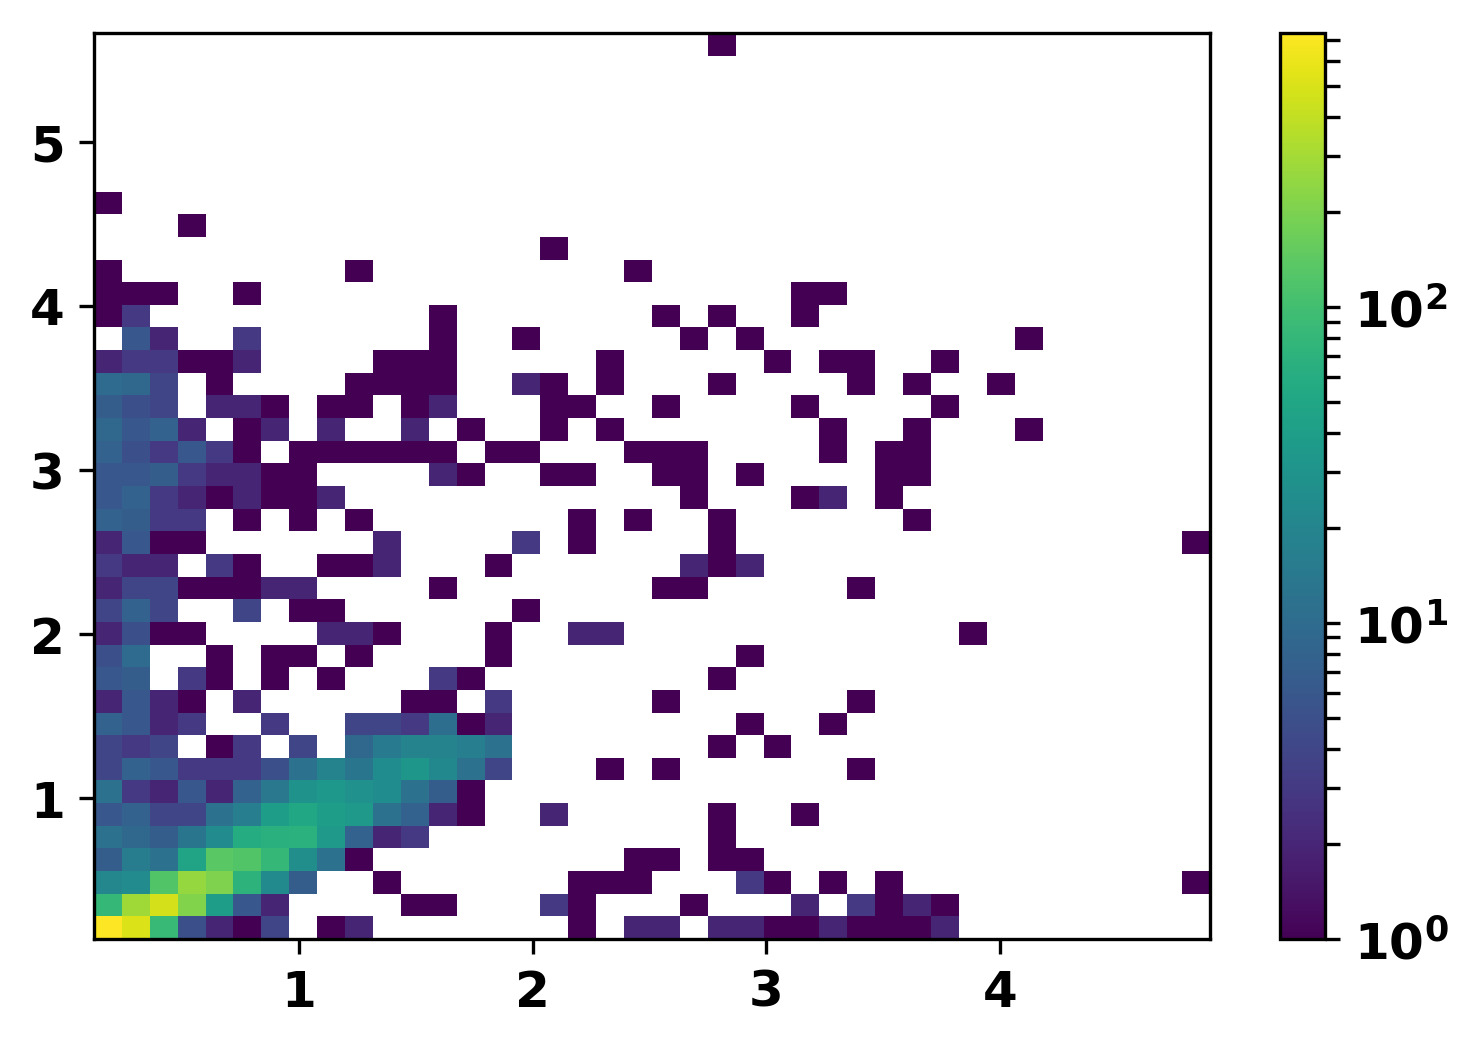
\includegraphics[clip,width=\textwidth]{Figs/act.png}
%\endminipage
%\minipage{0.33\textwidth}
%  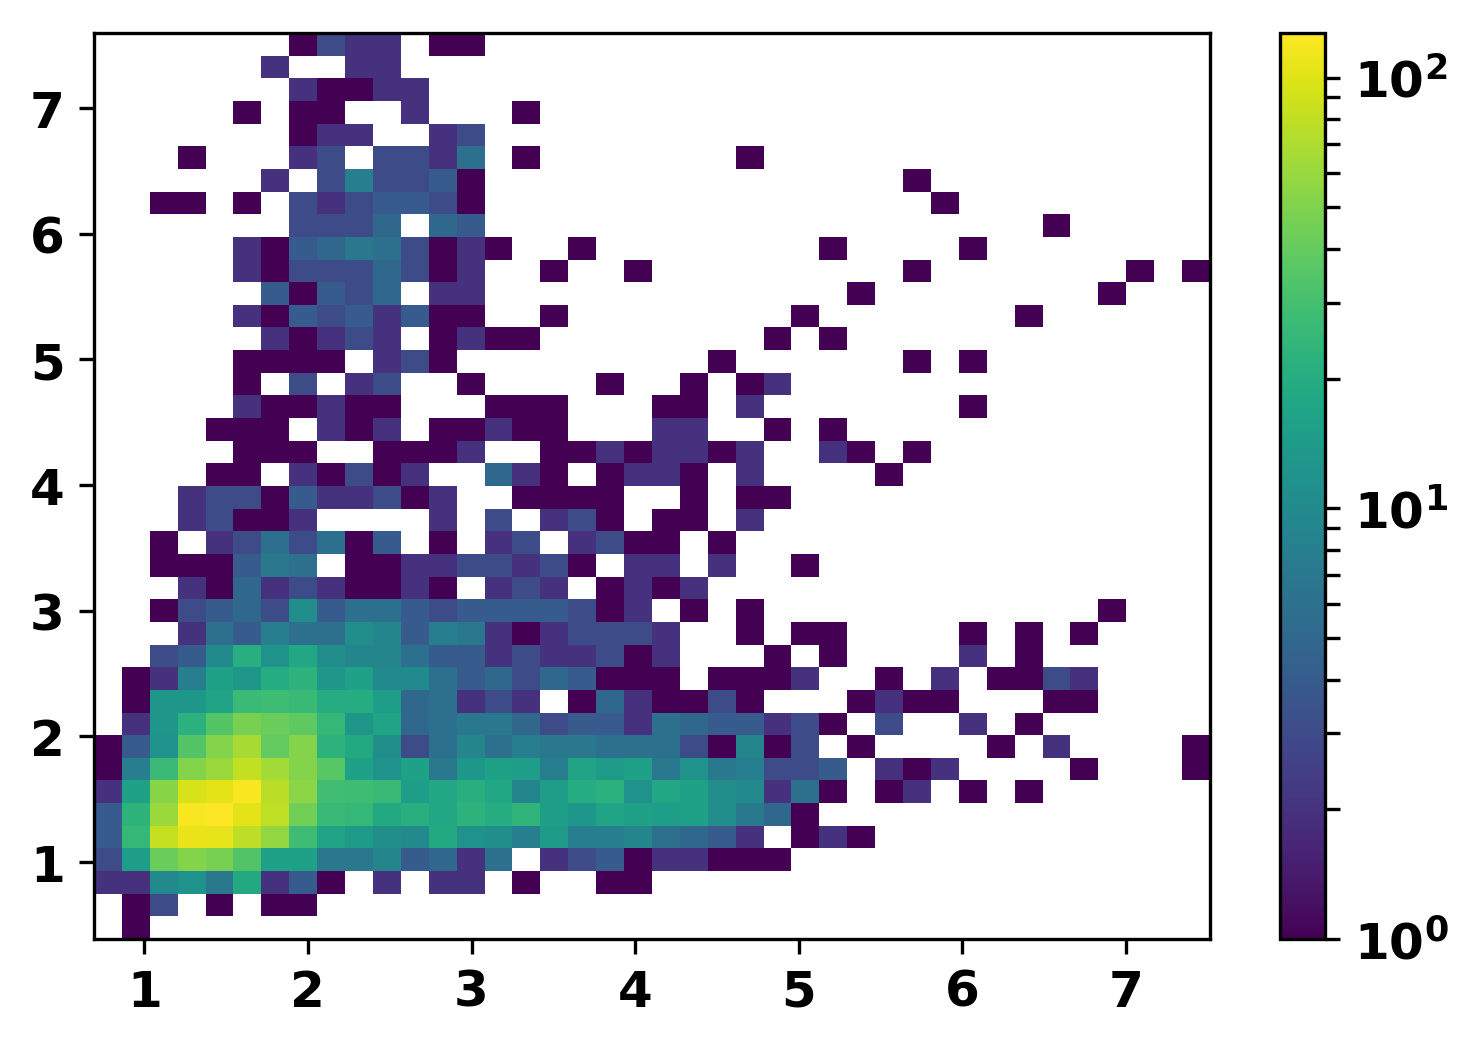
\includegraphics[clip,width=\textwidth]{Figs/in_act.png}
%  \endminipage
 %\minipage{0.33\textwidth}
%  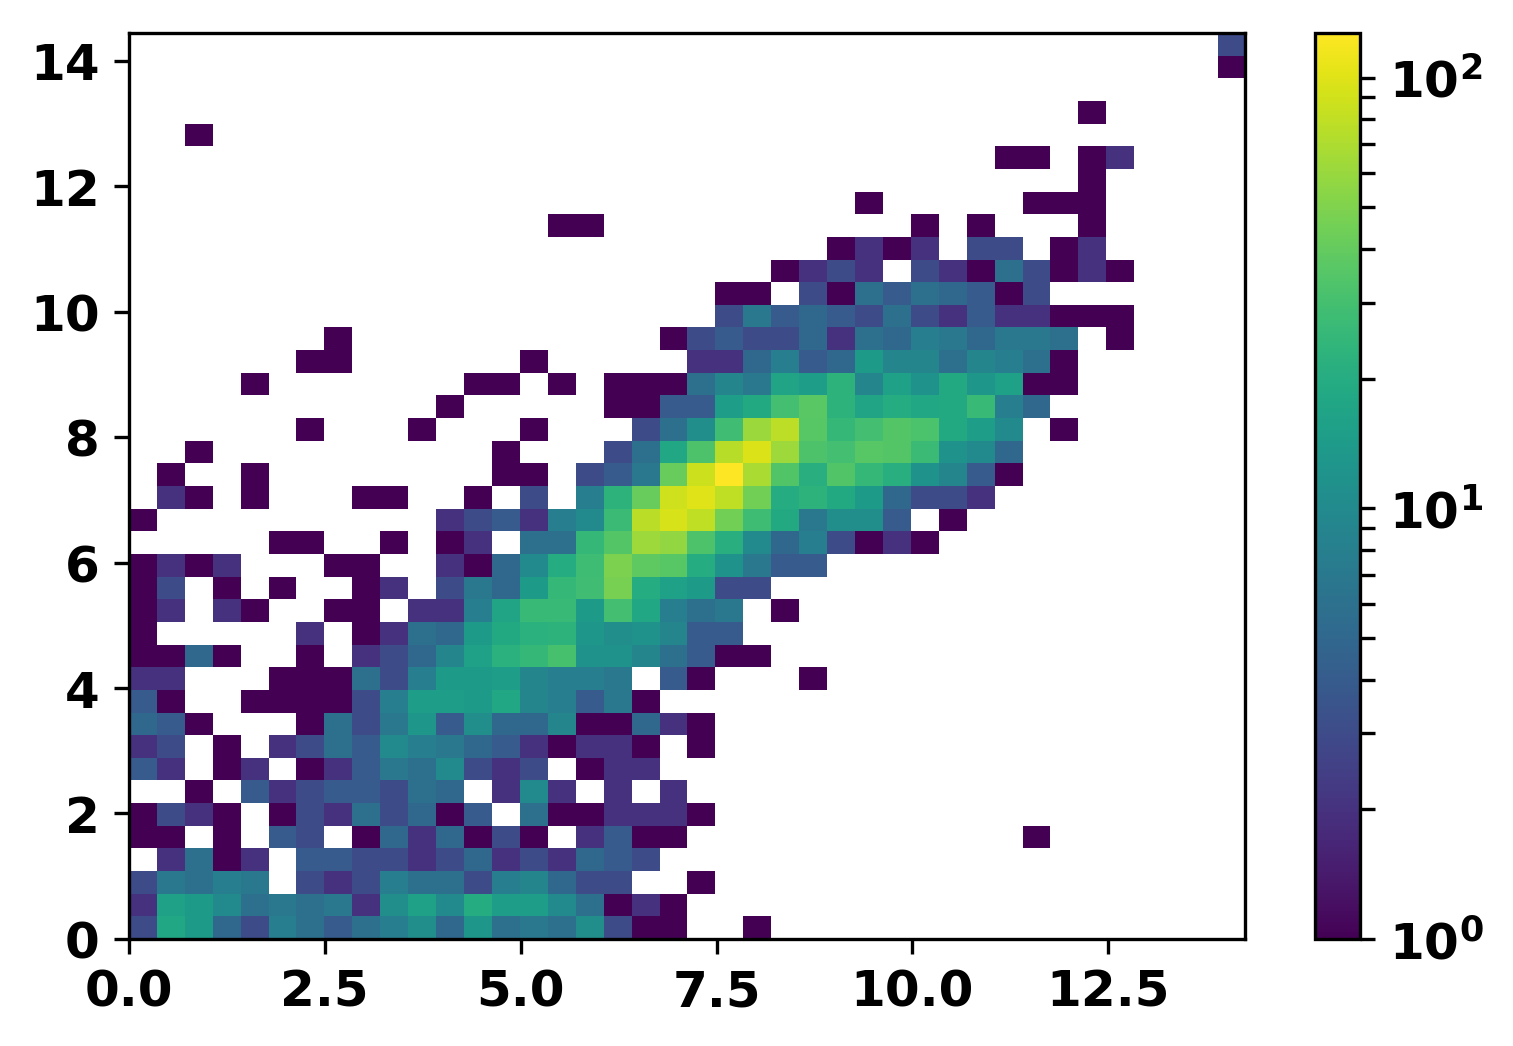
\includegraphics[clip,width=\textwidth]{Figs/t_rate.png}
%  \endminipage
%\captionof{figure}{2D histogram for bursting parameters of DD genes identified by scDDboost from dataset EMTAB2805 estimated by D3E. Left panel  : comparison of rate of promoter activation between two conditions, similarly, middle panel  : rate of promoter inactivation and right panel: rate of transcription when the promoter is in the active state. We observe that difference between transcription rate is smaller compare to difference between the activation and inactivation rate.}
%\end{figure}

%We observed that DD genes identified by scDDboost tends to have similar transcription rate when the promoter is active across condition, while there are lots of variabilities in the action and inactivation rate. Estimations from D3E reveals that the major factor to drive DD genes are activation and inactivation rate (proportions of different subtyps), it make sense to consider mixture model like scDDboost.



\section{Posterior consistency}
%\subsection{Posterior consistency}
%Under some parameters settings, the double dirichlet prior will have limited resolution and lead to inconsistency of posterior probabilities, which we investigate with the following asymptotic analysis.

%We first give the expression of posterior probability. Since there is no information favorable of any particular $A_\pi$, we select discrete uniform distribution as the prior for it, then the posterior probability is
%\begin{align}
%p(A_\pi | t^1, t^2) = c*\sum_{\pi' \text{ refines } \pi} p(t^1 | t^1_{\pi'})\, p(t^2 |  t^2_{\pi'} )
% \, p( t^1_{\pi'}, t^2_{\pi'} | A_{\pi'} )
%\end{align}
%for a normalizing constant $\frac{1}{c} = \underset{\pi' \in \Pi}\sum p(t^1 | t^1_{\pi'})\, p(t^2|  t^2_{\pi'} )
 %\, p( t^1_{\pi'}, t^2_{\pi'} | A_{\pi'} )$.
 
%Let $\Omega = \{(\phi, \psi): \overset{K}{\underset{i = 1}\sum}\phi_i = \overset{K}{\underset{i = 1}\sum}\psi_i = 1, \phi_i \geq 0, \psi_i \geq 0 , i = 1,..., K\}$ be the whole space. There is a subset of $\Omega$ we lack posterior inference. Let us first see an example:
%\begin{figure}[h]
%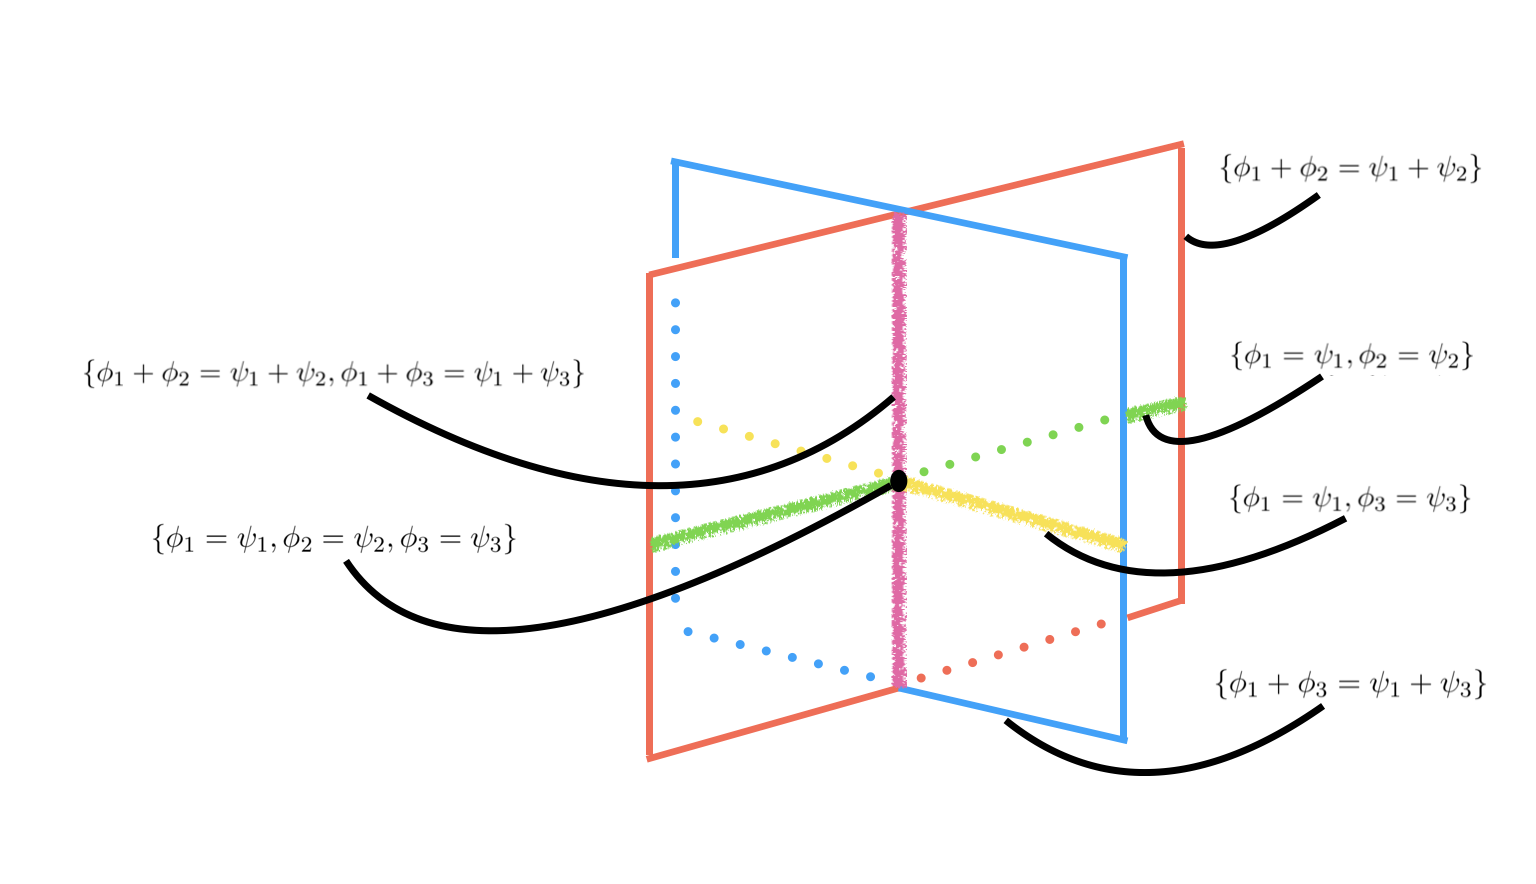
\includegraphics[scale = 0.5]{Figs/overlap.png}
% \caption{Four subtypes of cells,  simplexes of $(\phi,\psi)$ satisfying different constraints.}
%  \label{fig:1}
%\end{figure}
%\hfill\\
%In Fig 10, there are four subtypes, the rectangle with magenta boundary is a simplex $A_{\pi_1} = \{(\phi,\psi) : \phi_1 + \phi_2 = \psi_1 + \psi_2\}$, the rectangle with blue boundary is a simplex $A_{\pi_2} = \{(\phi,\psi) : \phi_1 + \phi_3 = \psi_1 + \psi_3\}$. The green line refers to $A_{\pi_3} = \{(\phi,\psi) : \phi_1 = \psi_1, \phi_2 = \psi_2\}$, the yellow line refers to $A_{\pi_4} = \{(\phi,\psi) : \phi_1 = \psi_1, \phi_3 = \psi_3\}$, the purple line refers to $A_{\pi_5} = \{(\phi,\psi) : \phi_1 + \phi_2 = \psi_1 + \psi_2, \phi_1 + \phi_3 = \psi_1 + \psi_3\}$, which is the intersection of $A_{\pi_1}$ and $A_{\pi_2}$, and finally the black dot which is the intersection of those three lines refers to the simplex with finest partitions, $\phi_i = \psi_i, \forall i = 1,..,4$. We lack posterior inference for $(\phi,\psi)$ along the purple line except the black dot. While on the green line, yellow line and black dot, we have consistent posterior inference(theorem 2). To explain why some space lacking posterior inference and define such space, we define a special subset $A_\pi^*$ of simplex $A_\pi$. $A_\pi^* = A_\pi\setminus \underset{\tilde{\pi} \text{ is not coarser than } \pi }\cup A_{\tilde{\pi}}$, $A_\pi^*$ is obtained by removing all intersection with other $A_{\tilde{\pi}}$(excluding those $A_{\tilde{\pi}}$ that is superset of $A_\pi$) from $A_\pi$. Since we removed those intersection parts. It is intuitive that $A_\pi^*$ will be disjoint subsets of $\Omega$.\\
%\begin{prop}
%if $\pi_1 \neq \pi_2$, then $A_{\pi_1}^*\cap A_{\pi_2}^* = \emptyset$
%\end{prop}
%\hfill\\
%Let $Q = \Omega\setminus \underset{\pi\in \Pi}\cup A_\pi^*$, and we have following proposition of the existence of $Q$.
%\begin{prop}
%Let $K$ be number of subtypes. When $K >  3, Q \neq \emptyset$, when $K \leq 3, Q = \emptyset$
%\end{prop}
%\hfill\\
%When the number of subtypes is bigger than three, we lack posterior inference on $Q$. To see that we can rewrite $A_\pi^*$ as $A_\pi^* = A_\pi\setminus \underset{\tilde{\pi} \text{ is not coarser than } \pi }\cup (A_{\tilde{\pi}}\cap A_\pi)$, $\tilde{\pi}$ is not coarser than $\pi$, which is equivalently to say $\pi$ is not refinement of $\tilde{\pi}$. By property 8 in section 2, $A_{\tilde{\pi}}\cap A_\pi$ is a lower dimensional subset of $A_\pi$. So $A_\pi \setminus A_\pi^*$ is a lower dimensional subset of $A_\pi$. For posterior on $Q$, it degenerates to integral on a lower dimensional subset of the simplex associating with densities, which will vanish\\
%\begin{prop}
%When $K >  3$, $p(Q | z^1, z^2) = 0$
%\end{prop}
%\hfill\\
%But for $(\phi, \psi)\in \Omega\setminus Q$, we have consistent posterior inference. %Assuming $\alpha_i^j = 1, \forall i$ in $1,2,...,K$, $j = 1,2$ and $\beta_b = \Sigma_{i\in b} (\alpha_i^1 + \alpha_i^2) = 2N(b)$, plug in (6) and integral on $A_\pi$ then we have simplified posterior
%\begin{align}
%p(A_\pi | y,z) = \frac{1}{c'}\sum_{\pi' \in \text{RF}(\pi)}\prod_{b\in \pi'}\frac{ \Gamma(\beta_b + t_b^1 + t_b^2)}{\Gamma(N(b) + t_b^1)\Gamma(N(b) + t_b^2)} \frac{\Gamma(N(b))}{\Gamma(2N(b))}
%\end{align}
%$c'$ is the total sum over all partitions $c' = \sum_{\pi}\prod_{b\in \pi}\frac{ \Gamma(\beta_b + t_b^1 + t_b^2)}{\Gamma(N(b) + t_b^1)\Gamma(N(b) + t_b^2)} \frac{\Gamma(N(b))}{\Gamma(2N(b))} $ And we have theorem 4.\\

%\begin{theorem} Let $n = min(n_1, n_2)$ be the smaller number of cells of two conditions and $n_1 = O(n_2)$ namely $\text{ln}(\frac{n_1}{n_2}) = 0$, and hyper parameters of DDM $\alpha^1, \alpha^2$ be vectors of constants, $\alpha_k^j \geq 1$, $\forall k, j$ and $\beta = \alpha^1 + \alpha^2$. Then if parameter $(\phi, \psi)\in \Omega\setminus Q $ we have 
%\begin{eqnarray*}
  %  p(A_{\pi} | y, z) \xrightarrow[n\rightarrow\infty]{\text{a.s.}}\left\{
    %            \begin{array}{ll}
      %           1 \quad \text{if }(\phi,\psi) \in A_\pi\\
        %         0 \quad \text{otherwise}\\             
          %      \end{array}
            %  \right.
%\end{eqnarray*}
%\end{theorem}
%\hfill\\
%Things become more complicate when $(\phi, \psi)$ falling into $Q$, we know $p(Q | y, z)$ vanishes, but $p(A_\pi | y,z)$ may not. 

%Recall $N(\pi)$ represents number of blocks $b$ in $\pi$. Let $S = \{\pi,  (\phi, \psi) \in A_\pi\}$, which is the collection of partitions whose associated simplexes covering $(\phi,\psi)$. Let $N^* = \underset{\pi\in S}\max$ $N(\pi)$, which is the max number of blocks of partitions from $S$. Let $S^* = \{\pi,  (\phi, \psi) \in A_\pi \text{ and } N(\pi) = N^*\}$, which is the collection of partitions that covering $(\phi, \psi)$ with number of blocks equal to the max number $N^*$. 

%For example, when $K = 7$, For a $(\phi, \psi)\in A_{\pi_1} \cap A_{\pi_2} \cap A_{\pi_3}$, $\pi_1 = \{\{1,2,3\}, \{4,5,6,7\}\}, \pi_2 = \{\{1,6,7\}, \{2,4\},\{3,5\}\}, \pi_3 = \{\{1,2,3,4,5,6\}\}$, and also $(\phi, \psi)$ does not belong to any other simplex $A_\pi$. Then $S = \{\pi_1, \pi_2, \pi_3\}$, $N^* = 3$, $S^* = \{\pi_2\}.$ 

%Denote components from right hand side of (5): $\frac{1}{c'}\underset{b\in \pi}\prod\frac{ \Gamma(\beta_b + t_b^1 + t_b^2)}{\Gamma(N(b) + t_b^1)\Gamma(N(b) + t_b^2)} \frac{\Gamma(N(b))}{\Gamma(2N(b))} = J(y,z,\pi).$  We have theorem 5.\\
%\begin{theorem} Following the setting in theorem 1, when parameter $(\phi, \psi)\in Q$,  and further if $\alpha^j, j = 1,2$ are vectors of integers, we have 
%\begin{eqnarray*}
%    (p(A_{\pi} | y, z))_{\pi\in S^*} \xrightarrow[n\rightarrow\infty]{\text{d}}%\left\{
                %\begin{array}{ll}
      %          (V_1, ..., V_{N(S^*)})
                 %m(\pi) \quad  \pi \in S^* \\
                 %0 \quad \text{otherwise}\\             
               % \end{array}
              %\right.
%\end{eqnarray*}
%and $\underset{\pi\in S^*}\sum m(\pi) = 1, m(\pi) > 0$\\
%$V_1, ..., V_{N(S^*)}$ are random variables and $V_1 + .. + V_{N(S^*)} = 1$
% \end{theorem} 

%Still using above example, in limiting case, we have $p(A_{\pi_3} | y,z) = 1$, $p(A_{\pi_2} | y,z) = 1$ and $p(A_{\pi_1}| y,z) = 0$. When the DE pattern is $B_{\pi_1}$ for some genes and our estimation of $p(A_{\pi_1}| y,z) = 0$, we will falsely classify those genes as differential distributed.

%The asymptotic properties help us gain insight of the performance of our approach,
%scDDboost may work poorly, when $(\phi, \psi)\in Q$, we may underestimate the posterior probability of true proportion change pattern, which reduce the posterior probabilities of true negative and enlarge false positive rate.\\






%\noindent
%{\bf Proofs:}

In this section, we proof theorem 4. 


As the density of DDM is computed by product or ratio over bunches of gamma function and gamma function is not easy to direct work on it and derive limiting theorem.
To proof theorem 4, we need a crucial lemma which gave us an approximation to the gamma function, namely

\begin{lemma}
For $x \geq 1$, $\frac{x^{x - c}}{e^{x - 1}} \leq \Gamma(x) \leq \frac{x^{x-1/2}}{e^{x - 1}}$, where $c = 0.577215...$ is the Euler-Mascheroni constant.
\end{lemma}

\begin{proof}
By \citep{ineq},  we have $\frac{x^{x - c}}{e^{x - 1}} \leq \Gamma(x) \leq \frac{x^{x-1/2}}{e^{x - 1}}$ for $x > 1$ and now we added the case when $x = 1, \Gamma(x) = 1$ so that both sides will include the equality case. 
\end{proof}


\begin{lemma}
For positive integer $n$, $\sqrt{2\pi} n^{n + 1/2}e^{-n} \leq \Gamma(n + 1) \leq e n^{n + 1/2}e^{-n}$ 
\end{lemma}



We have another two lemmas and theorem 1 and 2 are just proporsition of the lemma
\begin{lemma}
 If $(\phi, \psi) \in A_{\pi_1} \cap A_{\pi_2}$, follow the conditions in theorem 1 then 
 \begin{eqnarray*}
    \frac{\omega_{\pi_1}^{\text post}}{\omega_{\pi_2}^{\text post}} \xrightarrow[n\rightarrow\infty]{\text{a.s.}} 0 \quad \text{if } N(\pi_1) < N(\pi_2)\\
 \end{eqnarray*}
\end{lemma}


\begin{proof}
Recall $ \omega^{\rm post}_\pi \propto 
 p_\pi(t^1 | t^1_{\pi},y)\, p_\pi(t^2|  t^2_{\pi},y )
 \, p_\pi( t^1_{\pi}, t^2_{\pi} | y ) \, \omega_\pi.$
 and RHS $=  g(\pi, \alpha, \beta, n_1, n_2) f(\pi, t^1, t^2, \alpha, \beta)$ and $\frac{\omega_{\pi_1}^{\text post}}{\omega_{\pi_2}^{\text post}} = \frac{g(\pi_1, \alpha, \beta, n_1, n_2)}{g(\pi_2, \alpha, \beta, n_1, n_2)}\frac{f(\pi_1, t^1, t^2, \alpha, \beta)}{f(\pi_2, t^1, t^2, \alpha, \beta)}$
 where \begin{eqnarray*}
 g(\pi, t^1, t^2, \alpha, \beta) = \big[ \overset{2}{\underset{j = 1}{\prod}}\underset{b\in \pi}\prod \frac{\Gamma(\Sigma_{k\in b} \alpha_k^j)}{\prod_{k\in b} \Gamma(\alpha_k^j)} \big ] \frac{\Gamma(n_1 + 1) \Gamma(n_2 + 1)}{\prod_{b\in \pi} \Gamma(\beta_b)} \frac{\Gamma(\Sigma_{b \in \pi} \beta_b)}{\Gamma(n_1 + n_2 + \Sigma_{b\in\pi} \beta_b)}\\
f(\pi, t^1, t^2, \alpha, \beta) = \big[ \overset{2}{\underset{j = 1}{\prod}}\underset{b\in \pi}\prod \frac{1}{\prod_{k \in b}\Gamma(t_k^j + 1)}\frac{\prod_{k \in b}\Gamma(\alpha_k^j + t_k^j)}{\Gamma(t_b^j + \Sigma_{k\in b}\alpha_k^j)}\big ] \underset{b\in \pi}\prod \Gamma(\beta_b + t_b^1 + t_b^2) 
\end{eqnarray*}
For notation simplicity, we use the abbreviation $g(\pi), f(\pi)$ to substitute $g(\pi, \alpha, \beta, n_1, n_2),f(\pi, t^1, t^2, \alpha, \beta)$.  We take log on $\frac{\omega_{\pi_1}^{\text post}}{\omega_{\pi_2}^{\text post}}$, denote it as LR. $\text LR = \text{ln}g(\pi_1) - \text{ln}g(\pi_2) + \text{ln}f(\pi_1) - \text{ln}f(\pi_2)$. Denote $C(\pi_1, \pi_2, \alpha, \beta) = \text{ln}g(\pi_1) - \text{ln}g(\pi_2)$, $C(\pi_1, \pi_2, \alpha, \beta)$ does not change with sample size $n_1, n_2$ and is a constant determined by partition $\pi_1, \pi_2$ and hyper parameters $\alpha, \beta$.  For further convenience of notation let $h(x) = \text ln\Gamma(x)$ and $\gamma_b^j = \Sigma_{k\in b} \alpha_k^j$. Denote $R(\pi_1, \pi_2, t^1, t^2, \alpha, \beta) = \text{ln}f(\pi_1) - \text{ln}f(\pi_2)$. And removing the common part of $f(\pi_1)$ and $f(\pi_2)$, we have 
\begin{eqnarray*}
R(\pi_1, \pi_2, t^1, t^2, \alpha, \beta) = d(\pi_1, t^1, t^2, \alpha, \beta) - d(\pi_2, t^1, t^2, \alpha, \beta)\\
\end{eqnarray*}
where
\begin{eqnarray*}
d(\pi, t^1, t^2, \alpha, \beta) = \underset{b\in \pi}\Sigma h(\beta_b + t_b^1 + t_b^2) - \overset{2}{\underset{j = 1}{\Sigma}} \underset{b\in \pi}\Sigma h(t_b + \gamma_b^j)
\end{eqnarray*}


Recall $\beta_b = \gamma_b^1 + \gamma_b^2$ and from lemma 2, $(x - c)\text{ln}(x) - x + 1 \leq h(x) \leq (x - 1/2)\text{ln}(x) - x + 1$ we have 
\begin{align}
d(\pi, t^1, t^2, \alpha, \beta) &\geq \underset{b\in \pi}\Sigma (\beta_b + t_b^1 + t_b^2 - c) \text{ln}(\beta_b  + t_b^1 + t_b^2) - \overset{2}{\underset{j = 1}{\Sigma}}\underset{b\in\pi}\Sigma (t_b^j + \gamma_b^j - 1/2) \text{ln}(t_b^j + \gamma_b^j) + N(\pi)\\
d(\pi, t^1, t^2, \alpha, \beta) &\leq \underset{b\in \pi}\Sigma (\beta_b + t_b^1 + t_b^2 - 1 / 2) \text{ln}(\beta_b  + t_b^1 + t_b^2) - \overset{2}{\underset{j = 1}{\Sigma}}\underset{b\in\pi}\Sigma (t_b^j + \gamma_b^j - c) \text{ln}(t_b^j + \gamma_b^j) + N(\pi)
\end{align}


\begin{eqnarray*}
\text{RHS of (4)} = \Sigma_b \big[ (t_b^1 + \gamma_b^1) \text{ln}(1 + \frac{t_b^2 + \gamma_b^2}{t_b^1 + \gamma_b^1})
 + (t_b^2 + \gamma_b^2) \text{ln}(1 + \frac{t_b^1 + \gamma_b^1}{t_b^2 + \gamma_b^2})\\
 + (1 - c) \text{ln}(\beta_b + t_b^1 + t_b^2) 
  - 1/2(\text{ln}(1 + \frac{t_b^2 + \gamma_b^2}{t_b^1 + \gamma_b^1}) + \text{ln}(1 + \frac{t_b^1 + \gamma_b^1}{t_b^2 + \gamma_b^2}))\big] + N(\pi)
\end{eqnarray*}

By Taylor expansion at $x= 1$, $\text{ln}(x + 1) = \text{ln}2 + 1/2(x - 1) - 1/8(x - 1)^2 + g(\xi) (x - 1)^3$, where $g(\xi)$ is the reminder term of form $\frac{1}{3(1+\xi)^3}$ for $ 0 < \xi < x$
For a fixed $n_1, n_2$, we have 

\begin{eqnarray*}
\text{RHS of (4)} = (n_1 + n_2) \text{ln}2  - \Sigma_{b\in\pi}(1/8 (X_b^1 + X_b^2)\\
+ g(\xi_b) (Y_b^1 + Y_b^2) )+ T(\pi) + N(\pi)
\end{eqnarray*}

where $X_b^1 = \frac{(t_b^1 - t_b^2 + \gamma_b^1 - \gamma_b^2)^2}{t_b^1 + \gamma_b^1}$, $X_b^2 =  \frac{(t_b^1 - t_b^2 + \gamma_b^1 - \gamma_b^2)^2}{t_b^2 + \gamma_b^2}$,
$Y_b^1 = \frac{(t_b^1 - t_b^2 + \gamma_b^1 - \gamma_b^2)^3}{(t_b^1 + \gamma_b^1)^2} $ , $Y_b^2 =  \frac{(t_b^1 - t_b^2 + \gamma_b^1 - \gamma_b^2)^3}{(t_b^2 + \gamma_b^2)^2}$
and $T(\pi) = \Sigma_{b\in\pi}\big[(1 - c) \text{ln}(\beta_b + t_b^1 + t_b^2) 
  - 1/2(\text{ln}(1 + \frac{t_b^2 + \gamma_b^2}{t_b^1 + \gamma_b^1}) + \text{ln}(1 + \frac{t_b^1 + \gamma_b^1}{t_b^2 + \gamma_b^2}))\big]$\\
Similarly
\begin{eqnarray*}
\text{RHS of (5)} = (n_1 + n_2) \text{ln}2  -\Sigma_{b\in\pi}(1/8 (X_b^1 + X_b^2)\\
+ g(\xi_b) (Y_b^1 + Y_b^2)) + U(\pi) + N(\pi)
\end{eqnarray*}
  
$U(\pi) = \Sigma_{b\in\pi}\big[(2c - 1/2) \text{ln}(\beta_b + t_b^1 + t_b^2) 
  - c(\text{ln}(1 + \frac{t_b^2 + \gamma_b^2}{t_b^1 + \gamma_b^1}) + \text{ln}(1 + \frac{t_b^1 + \gamma_b^1}{t_b^2 + \gamma_b^2}))\big]$\\
  
 Using above inequalities, we have 
 \begin{eqnarray*}
% R(\pi_1, \pi_2, t^1, t^2, \alpha, \beta)  \geq T(\pi_1) - U(\pi_2) - 1/8 (\Sigma_{b\in\pi_1}(X_b^1 + X_b^2) - \Sigma_{b\in\pi_2}(X_b^1 + X_b^2)) \\ 
% - \Sigma_{b\in\pi_1}g(\xi_b)(Y_b^1 + Y_b^2)  - \Sigma_{b\in\pi_2}g(\xi_ b)(Y_b^1 + Y_b^2)\\
  R(\pi_1, \pi_2, t^1, t^2, \alpha, \beta)  \leq U(\pi_1) - T(\pi_2) - 1/8 (\Sigma_{b\in\pi_1}(X_b^1 + X_b^2) - \Sigma_{b\in\pi_2}(X_b^1 + X_b^2)) \\ 
 + \Sigma_{b\in\pi_1}g(\xi_b)(Y_b^1 + Y_b^2)  - \Sigma_{b\in\pi_2}g(\xi_ b)(Y_b^1 + Y_b^2)\\
 \end{eqnarray*}
 
 $Y_b^j =  \frac{((t_b^1 - t_b^2 + \gamma_b^1 - \gamma_b^2) / \sqrt{n}))^3 / \sqrt{n}}{((t_b^j + \gamma_b^j) /n)^2}$, by LLN the denominator goes to a constant and by CLT in the numerator $(t_b^1 - t_b^2 + \gamma_b^1 - \gamma_b^2) / \sqrt{n} \rightarrow (t_b^1 - t_b^2) / \sqrt{n} \rightarrow \sqrt{n}[(t_b^1 / n  - \Phi_b) - (t_b^2 / n - \Psi_b)] $, which goes to a normal distributed random variables when $\Phi_b = \Psi_b$. So $Y_b^j$ is $o_p(1)$. Similarly,  $X_b^j =  \frac{((t_b^1 - t_b^2 + \gamma_b^1 - \gamma_b^2) / \sqrt{n})^2}{t_b^j + \gamma_b^j / n}}$ is asymptotic gamma($\chi$-square) distributed.
$g(\xi_b)$ has bounded variance,
 $U(\pi_1) - T(\pi_2) = -\text{ln}(n)$ if $N(\pi_2) < N(\pi_1)$
 as $ \text{ln}(\beta_b + t_b^1 + t_b^2)  -  \text{ln}(\beta_{b'} + t_{b'}^1 + t_{b'}^2) =  \text{ln}(\frac{\beta_b + t_b^1 + t_b^2}{n})  -  \text{ln}(\frac{\beta_{b'} + t_{b'}^1 + t_{b'}^2}{n}) \rightarrow O(1) \quad a.s.$ so we complete the proof

%Recall $t^1 \sim \text{multinomial}(n_1, \phi)$, $t^2 \sim \text{multinomial}(n_2, \psi)$.



\end{proof}


\begin{lemma}
 If $(\phi, \psi) \in A_{\pi_1} \cap A_{\pi_2}$, follow the conditions in theorem 1 and further we have $\alpha^j, j = 1,2$ be vectors of integers then 
\begin{eqnarray*}
 \frac{\omega_{\pi_1}^{\text post}}{\omega_{\pi_2}^{\text post}} \xrightarrow[n\rightarrow\infty]{\text{d}} v \quad \text{if } N(\pi_1) = N(\pi_2)\\
\end{eqnarray*}
$v$ is a random variable
\end{lemma}

\begin{proof}
follow almost same procedure in lemma 4, but instead of using inequalities in lemma 2, we use lemma 3. And we still have
\begin{eqnarray*}
d(\pi, t^1, t^2, \alpha, \beta) = \underset{b\in \pi}\Sigma h(\beta_b + t_b^1 + t_b^2) - \overset{2}{\underset{j = 1}{\Sigma}} \underset{b\in \pi}\Sigma h(t_b + \gamma_b^j)
\end{eqnarray*}
and by lemma 3
\begin{align}
d(\pi, t^1, t^2, \alpha, \beta) &\geq \underset{b\in \pi}\Sigma (\beta_b + t_b^1 + t_b^2 - 1/2) \text{ln}(\beta_b  + t_b^1 + t_b^2) - \overset{2}{\underset{j = 1}{\Sigma}}\underset{b\in\pi}\Sigma (t_b^j + \gamma_b^j - 1/2) \text{ln}(t_b^j + \gamma_b^j) + \text{ln}(\sqrt{2\pi}) - 1\\
d(\pi, t^1, t^2, \alpha, \beta) &\leq \underset{b\in \pi}\Sigma (\beta_b + t_b^1 + t_b^2 - 1/2) \text{ln}(\beta_b  + t_b^1 + t_b^2) - \overset{2}{\underset{j = 1}{\Sigma}}\underset{b\in\pi}\Sigma (t_b^j + \gamma_b^j - 1/2) \text{ln}(t_b^j + \gamma_b^j) + 1 - \text{ln}(\sqrt{2\pi})
\end{align}

\begin{eqnarray*}
R(\pi_1, \pi_2, t^1, t^2, \alpha, \beta)  \approx D(\pi_1) - D(\pi_2) - 1/8 (\Sigma_{b\in\pi_1}(X_b^1 + X_b^2) - \Sigma_{b\in\pi_2}(X_b^1 + X_b^2)) \\ 
 - \Sigma_{b\in\pi_1}g(\xi_b)(Y_b^1 + Y_b^2)  - \Sigma_{b\in\pi_2}g(\xi_ b)(Y_b^1 + Y_b^2)\\
\end{eqnarray*}
where $D(\pi) = \Sigma_{b\in\pi}\big[1/2 \text{ln}(\beta_b + t_b^1 + t_b^2) 
  - c(\text{ln}(1 + \frac{t_b^2 + \gamma_b^2}{t_b^1 + \gamma_b^1}) + \text{ln}(1 + \frac{t_b^1 + \gamma_b^1}{t_b^2 + \gamma_b^2}))\big]$
And $D(\pi_1) - D(\pi_2)$ is O(1) if $N(\pi_1) = N(\pi_2)$ as $ \text{ln}(\beta_b + t_b^1 + t_b^2)  -  \text{ln}(\beta_{b'} + t_{b'}^1 + t_{b'}^2) =  \text{ln}(\frac{\beta_b + t_b^1 + t_b^2}{n_1})  -  \text{ln}(\frac{\beta_{b'} + t_{b'}^1 + t_{b'}^2}{n_1}) \rightarrow 0 \quad a.s.$


\end{proof}



\hfill\\
Proof of theorem 4 
\begin{proof}

Recall $\sum_{\pi \in \Pi} \omega^{\rm post}_{ \pi} = 1$ and $P(A_\pi|y,z) = 
\sum_{\tilde \pi \in \Pi} \omega^{\rm post}_{\tilde \pi} \,  1[ {\mbox {\rm $\tilde \pi$ refines $\pi$}} ].$  If $(\phi, \psi) \notin \text{Q}$, for all the $A_\pi$ covers $(\phi, \psi)$ there is one finest $\pi^*$ with the largest $N(\pi^*)$ and every other $\pi$ that $(\phi,\psi) \in A_\pi$ is coarser than $\pi^*$. We get the results of theorem 4 by lemma 4.

%Similarly we use lemma 5 could proof theorem 5. 

\end{proof}

%Given the condition that $\alpha_k = 1, \forall k$ and $\beta_b = \sum_{k\in b} \alpha_k$, recall $p(A_\pi| y,z) = \sum_{\pi' \in \text{RF}(\pi)} J(y,z,\pi')$  and $ J(y,z,\pi) = \frac{1}{c'}\underset{b\in \pi}\prod\frac{ \Gamma(\beta_b + t_b^1 + t_b^2)}{\Gamma(N(b) + t_b^1)\Gamma(N(b) + t_b^2)} \frac{\Gamma(N(b))}{\Gamma(2N(b))}$\\
%Assuming there are $K$ subgroups, since $n_1$ and $n_2$ goes to infinite at same rate, for simplicity we assume $n_1 = n_2$, and the multiplicity term $\frac{\Gamma(N(b))}{\Gamma(2N(b))}$ in $J(y,z,\pi)$ remains finite for any $\pi$. To demonstrate limiting 
%$t^1\sim \text{multinomial}(\phi), t^2\sim \text{multinomial}(\psi)$ 
%$t_b^1 = \sum_{i \in b} z_i^1$ and $t_b^2 = \sum_{i \in b} z_i^2$, so $t_b^1 \sim$ binomial $(n, \Phi_b)$ and $t_b^2 \sim$ binomial $(n, \Psi_b)$, where $\Phi_b = \sum_{i \in b}\phi_i$ and $\Psi_b = \sum_{i \in b}\psi_i$. Let $f(n, b) = \frac{\Gamma(\beta_b + t_b^1 + t_b^2)}{\Gamma(\beta_b + t_b^1)\Gamma(\beta_b + t_b^2)}$, then 
%$$J(z^1, z^2 ,\pi) \propto \prod_{b\in \pi} f(n,b)$$\\
l%og$f(n, b) = $log$(\Gamma(\beta_b + t_b^1 + t_b^2))$ - log$(\Gamma(\beta_b + t_b^1))$ - log$(\Gamma(\beta_b + t_b^2))$, notice that $t_b^1, t_b^2 \text{ and } \beta_b$ are integers, and when $x$ is integer,  $\Gamma(x)$ is the factorial of $(x - 1)$.
%We have log$f(n, b) = $log$((\beta_b + t_b^1 + t_b^2 -1)!) - \text{log}((\beta_b + t_b^1 -1)!) - \text{log}((\beta_b + t_b^2 -1)!)$  and when $n$ is large we could use Stirling's approximation, i.e. log$(n!)$ = $n$log$(n) - n + O(\text{log}(n))$, we have log$((\beta_b + t_b^1 + t_b^2 -1)!) - \text{log}((\beta_b + t_b^1 -1)!) - \text{log}((\beta_b + t_b^2 -1)!)\approx (\beta_b + t_b^1 + t_b^2-1)\text{log}(\beta_b + t_b^1 + t_b^2-1) - (\beta_b + t_b^1 -1)\text{log}(\beta_b + t_b^1 -1) - (\beta_b + t_b^2 -1)\text{log}(\beta_b + t_b^2 -1) + O(\text{log}(n))$.\\
%Plug into $f(n,b)$ we have:\\
%$$\text{log}f(n,b) \approx (\beta_b + t_b^1 -1)\text{log}(1 + \frac{t_b^2}{\beta_b + t_b^1 -1}) + (\beta_b + t_b^2 -1)\text{log}(1 + \frac{t_b^1}{\beta_b + t_b^2 -1}) + O(\text{log}(n))$$\\
%as $\beta_b \text{log}(\beta_b + t_b^1 + t_b^2 -1) \sim O(\text{log}(n))$ and by law of large number and slutsky's theorem, $\text{log}(1 + \frac{t_b^2}{\beta_b + t_b^1 -1}) \rightarrow \text{log}(1+\frac{\Psi_b}{\Phi_b})$,
%$\text{log}(1 + \frac{t_b^1}{\beta_b + t_b^2 -1}) \rightarrow \text{log}(1+\frac{\Phi_b}{\Psi_b})$ $a.s.$ and $\frac{\text{log}f(n, b)}{n} \rightarrow \Phi_b\text{log}(1+\frac{\Psi_b}{\Phi_b}) + \Psi_b\text{log}(1+\frac{\Phi_b}{\Psi_b})$ a.s. We have:\\
%$$ \frac{\text{log}(\prod_{b\in \pi} f(n,b))}{n} \rightarrow \sum_b [\Phi_b\text{log}(1+\frac{\Psi_b}{\Phi_b}) + \Psi_b\text{log}(1+\frac{\Phi_b}{\Psi_b})] \quad a.s.$$
%To find the maxima $(\Phi, \Psi)$, we fix $\Psi$ and 
%let $C =  \frac{\text{log}(\prod_{b\in \pi} f(n,b))}{n} + \lambda(\underset{b\in\pi}\sum \Phi_b - 1)$, we have $\frac{\partial C}{\partial \Phi_b} =  \text{log}(1+\frac{\Psi_b}{\Phi_b}) + \lambda$, stationary point is $\Phi_b = \Psi_b, \forall b$. and for the hessian matrix $\frac{\partial^2 C}{\partial \Phi_b^2} = -%\frac{\Psi_b}{\Phi_b^2 + \Phi_b\Psi_b} < 0$ and $\frac{\partial^2 C}{\partial \Phi_{b}\partial \Phi_{b'}} = 0, \text{if } b \neq b'$, that is to say the hessian matrix is a diagonal matrix with every diagonal elements to be negative, so it is negative definite, and our objective function is concave. The maxima is the stationary point $\Phi = \Psi$. 
%And when $\Phi = \Psi$ , $\frac{\text{log}(\prod_{b\in \pi} f(n,b))}{n} = 2\text{ln}(2)$ a constant not dependent on partition $\pi$ and $\Phi$. That is to say if $(\phi,\psi) \in A_{\pi_1}\cap A_{\pi_2}$ and $(\phi,\psi) \notin A_{\pi_3}$. Then we would have 
%$\lim_{n\to\infty}\frac{\text{log}(\prod_{b\in \pi_1} f(n,b))}{n} = \lim_{n\to\infty}\frac{\text{log}(\prod_{b\in \pi_2} f(n,b))}{n}$ and  $\lim_{n\to\infty}[\frac{\text{ln}(\prod_{b\in \pi_1} f(n,b))}{n} -  \frac{\text{log}(\prod_{b\in \pi_3} f(n,b))}{n}]  = c > 0 $, which implies:
%\[\frac{J(t^1, t^2,\pi_3)}{J(t^1, t^2,\pi_1)} \rightarrow 0\quad a.s. \tag{A}\]
%To investigate the limit of $\frac{J(t^1, t^2,\pi_1)}{J(t^1, t^2,\pi_2)}$, We use inequalities that $\sqrt{2\pi}n^{n+\frac{1}{2}}e^{-n} \leq n! \leq en^{n+\frac{1}{2}}e^{-n}$ holds for all nonnegative integers $n$. Plug in $f(n,b)$, we have:\\
%\[
%\beta_b +\text{log}\sqrt{2\pi} - 3 + g(n,b) 
%\leq f(n, b)\leq
%\beta_b - 2\text{log}\sqrt{2\pi} + g(n, b)\tag{1}
%\]\\
%\[g(n,b) =  (\beta_b + t_b^1 - \frac{1}{2})\text{log}(1 + \frac{t_b^2}{\beta_b + t_b^1 -1}) + (\beta_b + t_b^2 - \frac{1}{2})\text{log}(1 + \frac{t_b^1}{\beta_b + t_b^2 -1}) - (\beta_b - \frac{1}{2})\text{log}(\beta_b + t_b^1 + t_b^2 - 1)\]\\
%Based on inequalities (1), $\underset{{b\in\pi}}\sum f(n,b)$ only differ with $\underset{b\in\pi}\sum g(n,b)$ by a constant.
%By Taylor's expansion $\text{log}(1+x) = \text{log}2 + \frac{1}{2}(x - 1) + O( (x-1)^2)$, we have $\text{log}(1 + \frac{t_b^2}{\beta_b + t_b^1 -1}) = \text{log}2 + \frac{1}{2}(\frac{t_b^1 - t_b^2 + 1 - \beta_b}{\beta_b + t_b^1 -1}) + O_p((\frac{t_b^1 - t_b^2 + 1 - \beta_b}{\beta_b + t_b^1 -1})^2)$ and under condition $\Phi_b = \Psi_b, \frac{(t_b^1 - t_b^2 + 1 - \beta_b)^2}{\beta_b + t_b^1 -1}$ is $O_p(1)$. Plug in $g(n,b)$\\
%$$g(n,b) = \text{log}2 * t_b^1 + \text{log}2 * t_b^2  - (\beta_b - \frac{1}{2})\text{log}(\beta_b + t_b^1 + t_b^2 - 1) + O_p(1) $$
%and sum up 
%\[\sum_{b\in\pi} g(n,b) = 2n\text{log}2 - \sum_{b\in\pi}(\beta_b - \frac{1}{2})\text{log}(\beta_b + t_b^1 + t_b^2 - 1) + O_p(1)  \tag{2} \]
%Notice that when two partition $\pi_1$, $\pi_2$ have same number of blocks $b$ and $\Phi_b = \Psi_b$, $\forall b \in \pi_1\cup\pi_2$, 
%\begin{align*}
%\sum_{b\in\pi_1} g(n,b) - \sum_{b'\in\pi_2} g(n,b') &= \sum_{b'\in\pi_2}(\beta_b' - \frac{1}{2})\text{log}(\beta_b' + t_{b'}^1 + t_{b'}^2 - 1) - \sum_{b\in\pi_1}(\beta_b - \frac{1}{2})\text{log}(\beta_b + t_b^1 + t_b^2 - 1) +  O_p(1)\\
%&= \sum_{b'\in\pi_2}(\beta_{b'}- \frac{1}{2})\text{log}(\frac{\beta_b' + t_{b'}^1 + t_{b'}^2 - 1}{n}) -  \sum_{b\in\pi_1}(\beta_b - \frac{1}{2})\text{log}(\frac{\beta_b + t_b^1 + t_b^2 - 1}{n})\\
% &+ \sum_{b'\in\pi_2 - \frac{1}{2}}(\beta_{b'}  - \frac{1}{2})\text{log}(n) - \sum_{b\in\pi_1 - \frac{1}{2}}(\beta_b - \frac{1}{2})\text{log}(n) + O_p(1)\\
%&= O_p(1) + \sum_{b\in\pi_1}\frac{1}{2}\text{log}(n) - \sum_{b'\in\pi_2}\frac{1}{2}\text{log}(n) \\
%&= O_p(1)
%\end{align*}
%When $\pi_1$ and $\pi_2$ have same number of blocks,  
%\[\frac{J(t^1, t^2,\pi_1)}{J(t^1, t^2,\pi_2)} \rightarrow O_p(1)\quad a.s. \tag{B}\]
%When $\pi_1$ have less blocks than $\pi_2$, $\sum_{b'\in\pi_2} g(n,b') - \sum_{b\in\pi_1} g(n,b) = O_p(\text{log}(n))$
%\[\frac{J(t^1, t^2,\pi_1)}{J(t^1, t^2,\pi_2)} \rightarrow 0\quad a.s.\tag{C}\]

%\bibliographystyle{IEEEtran}
\bibliographystyle{imsart-nameyear}
\bibliography{./supp_references/wlr_ref}





\end{document}  
